\documentclass[12pt, a4paper]{report}   	% use "amsart" instead of "article" for AMSLaTeX format
\usepackage[utf8]{inputenc} %æøå


\usepackage{geometry}                		% See geometry.pdf to learn the layout options. There are lots.
\geometry{letterpaper}                   		% ... or a4paper or a5paper or ... 

\usepackage[parfill]{parskip}    		% To begin paragraphs with an empty line rather than an indent

%Tables
\usepackage[none]{hyphenat}  % Stops breaking up words in a table
\usepackage{array}

%Img
\usepackage{graphicx}				% To import images
\usepackage{float}						% Control of float positions

\usepackage{hyperref} % Clicable references
\hypersetup{hidelinks, urlcolor=cyan}									
\usepackage{amssymb}

%Nice looking kode
\usepackage{listings}
\lstset{literate=%
{æ}{{\ae}}1
{å}{{\aa}}1
{ø}{{\o}}1
{Æ}{{\AE}}1
{Å}{{\AA}}1
{Ø}{{\O}}1
}

%Nice looking chapters
\usepackage[T1]{fontenc}
\usepackage{titlesec, blindtext, color}
\definecolor{gray75}{gray}{0.75}
\newcommand{\hsp}{\hspace{20pt}}
\titleformat{\chapter}[hang]{\Huge\bfseries}{\thechapter\hsp\textcolor{gray75}{|}\hsp}{0pt}{\Huge\bfseries}

\title{Micro tasking, an efficient method for data acquisition for digital maps?}
\author{Anne Sofie Strand Erichsen}
%\date{}							% Activate to display a given date or no date

\begin{document}

%Front stuff
\pagenumbering{roman}

\maketitle

%Table of contents with no page number
\tableofcontents   
\thispagestyle{empty}
\cleardoublepage

%List of figures, list of tables
\setcounter{page}{1}
%\listoffigures
%\addcontentsline{toc}{section}{\numberline{}List of Figures}
\cleardoublepage

%\listoftables
%\addcontentsline{toc}{section}{\numberline{}List of Tables}
%\cleardoublepage

%Main document and numbering starts here
\pagenumbering{arabic}

\setcounter{page}{1}


\abstract
TB!
%A big problem with OSM is finding a good, fast and easy way of correcting data. There exists multiple tools that finds possible errors, but there also has to be a good way of fixing them. A solution to this problem can be can be microtasking. Microtasks are formed basically by dividing a project into smaller tasks, clearly defined, that can be performed independently \cite{EstellesArolas}.  

\chapter{Introduction}\label{sec:intro}

Voluntary acquisition of data for digital mapping has become quite popular over the last years. This is also a cornerstone for Open Street Map (OSM), which is a global open access database for digital maps. To establish data sets (for maps) is a comprehensive task. By dividing the work into many small sub-tasks, each of these tasks may be possible to handle by voluntary enthusiasts. This is called Microtasking.

The Norwegian government has indicated that the most detailed map data for Norway (FKB) may become freely available within a few years. If so, these data may be included in the database of OSM.   

\textit{During this paper the student is suppose to:} \\
- Study relevant literature \\
- Study how Microtasking is working \\
- Explore how data from FKB can be mapped into OSM \\
- Investigate if Microtasking is a possible method for including FKB in OSM \\


%This paper will inform you on the technical challenges regarding OpenStreetMap and governmental data \cite{Exel2010}. For a summary of papers you can see on page \pageref{sec:wang}

%In theory micotasking seems to solve a lot of OSM problems like overlapping data, deletion of good metadata (read: tags) when running import-scripts and makes it easier to control, both the workflow and quality of the data. Microtasking splits a task into multiple subtasks and distributing these subtasks to humans over the internet.  The OSM mindset  of schema-less datasets and tags differs from many organizations. With the success of OSM it is time to start taking this mindset serious. OSM also has its weaknesses , but many people believe microtasking solves the majority of them. By using FKB building dataset I will try too look further into mapping governmental data over to the OSM format, also trying to experience if microtasking is the solution of the weaknesses of OSM, like the ones I mentioned above. 


\chapter{Motivation}
There are two types of people in the free and open source software for Geoinformatics community: First type are they who has an geomatics background and learned ICT afterwards and second type are they who has an ICT background and learned geomatics on their own afterwards. The last type has a much higher percentage in the community. 

%Importing FKB data into OpenStreetMap would increase the coverage in Norway tremendously.... 
An import of FKB data could result in a 3D modell of the entire country, free and available for everyone. FKB contain very detailed building data and gives a good foundation for 3D modelling of buildings. Trondheim will be a test municipality in this paper. Here buildings are added manually by users drawing manually over aerial photos. Height and roof shape are not added, making 3D modelling of buildings very difficult. An example of 3D modeling of buildings in Trondheim added manually from aerial photo is shown in figure \ref{fig:3Dekstrd}.

\begin{figure}[H]
    \centering
    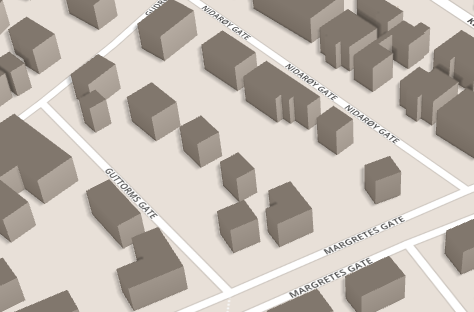
\includegraphics[scale=0.4]{figures/FixedByMe/3DmodellTRD.png}
    \caption{3D modeling of buildings in Trondheim, source: osmbuildings.org}
    \label{fig:3Dekstrd}
\end{figure}  

The same buildings 3D modeled with building data from FKB is shown in figure \ref{fig:3DekstrdFKB}. This model is created by Norkart. 

\begin{figure}[H]
    \centering
    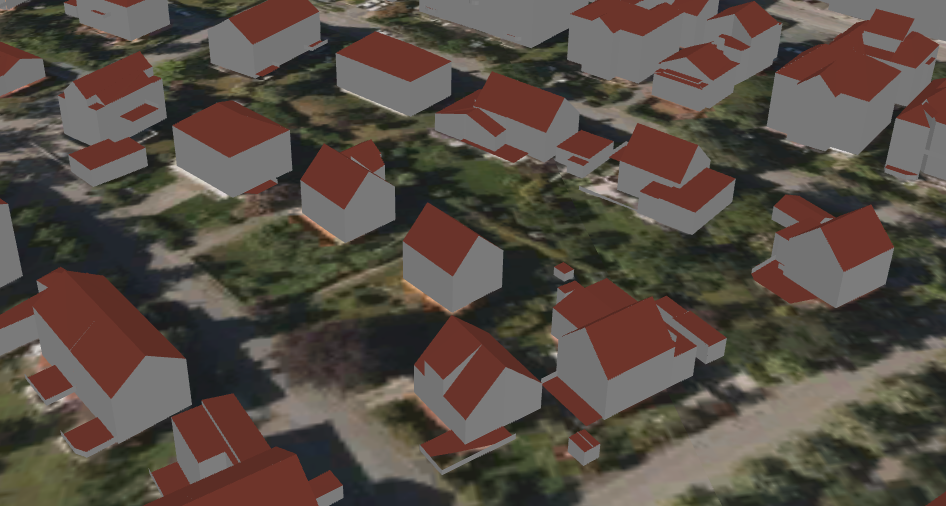
\includegraphics[scale=0.4]{figures/FixedByMe/3DmodelTRD-FKB.png}
    \caption{3D modeling of buildings in Trondheim, source: 3d.kommunekart.com}
    \label{fig:3DekstrdFKB}
\end{figure}  

Importing data into OSM is not easy. Finding the most optimal approach is not easy. An import should follow the OSM import guidelines. Finding a balance between manual verification and automatic import is not easy. The import should require more work than a manual import. Here is the micro-tasking method maybe a solution. Two big building imports has used this method and this paper will look at how they did it, and how it worked and what didn't work. 

%\chapter{Technical}

\subsection{Existing libraries}
The internet consists of hundreds of software libraries and packages. It can be overwhelming for newcomers and hard to find the most suited ones. A good tip is to learn the handful of libraries and packages that most software is derived from, so called root libraries. They are actively maintained and not significantly derived from any other libraries. The libraries do geospatial operations that are hard to implement, so people choose to use the libraries instead. Geospatial datasets are large, often complex and varied. This makes the implementation harder, and some of the reasons for the libraries success. The root libraries are GDAL, OGR, GEOS and PROJ. 4 \cite{Lawhead2013}.  They are, according to J. Lawhead, "the heart and soul of of the geospatial analysis community". All the libraries are written in C or C++. 




%\chapter{OSM import methods}
%1. Helautomatisk, scriptet import \\
%2. Helmanuell import basert p� tracing av f.eks WMS-data\\
%3. Guidet automatisk import (slik import av n50-data blir gjort i OSM i dag) \\
%4. Import basert p� metodikken LA-buildings-prosjektet har gjort, og som beskrives av McAndrews (microtasking)

%Conflation \href{http://wiki.openstreetmap.org/wiki/Conflation}{Wiki Conflation}
\subsection{Introduction}
The traditional way to contribute data to the OpenStreetMap project is through active users who use their GPS to track roads and their local knowledge to add information about their geographic regions to the OSM database \cite{Zielstra2013}. Users also digitalize aerial photos. Cheaper GPS receivers and more available satellite imagery with better resolution makes it easier for users to contribute \cite{Chilton}. The number of active users in different regions varies a lot, making some areas on the OSM map full of data while others are almost empty. This led to a second approach for getting data in to the OpenStreetMap database, bulk imports \cite{Zielstra2013}.  Bulk imports is the process of uploading external data and were meant for initial/preliminary object class uploads, so only if the object were none existing in the area  \cite{Zielstra2013}.  Its a good alternative for countries or regions with less active users. Through the years different import methods has been developed. This paper will evaluate the most common methods. 

\subsection{Fully automatic import script}
Creating a script that automatically imports big datasets into OpenStreetMap, a bulk import, is not encouraged in the OSM community \cite{Zielstra2013}. This becomes clear when reading the wikipages about import. A bulk import is suppose to be a supplement to user generated data. The user generated data and the users ability to work is always the priority \cite{OSMimport}. Automatic edits is changes that has no or very limited human oversight \cite{OSMAutiEdit}. This kind of edits must follow the Automated Edits code of conduct \cite{OSMAutomaticEdits}. A fully automatic import do automated edits to the OpenStreetMap database with little, if any, verification from a human. 

An example of a bulk import was the TIGER import. The Topologically Integrated Geographical Encoding and Reference system (TIGER) data was produced by the US Census Bureau and is a public domain data source. The bulk import was completed in early 2008 \cite{Zielstra2013}, populating the nearly empty map of the United States. The TIGER data was not perfect and had it's faults, but it was better than no data at all \cite{Willis2008}. 

On the TIGER OpenStreetMap wikipage, last updated August 2016, they say it is unlikely that the TIGER data ever will be imported again. The main reason is the growing US mapping community, their mapping is often better than the TIGER data. "Do not worry about getting your work overwritten by new TIGER data. Go map!" \cite{WikiOSMTIGER2007}. A new bulk import with updated TIGER data can overwrite existing, more precise data. The TIGER data are of variable quality, poor road alignment is a huge problem and also wrong highway classification. Many hours of volunteer work could be lost and this is something the community want to avoid. The bulk import in 2007 got the United States on the OSM-Map and saved the mapping community a lot of time finding road names etc. "TIGER is a skeleton on which we can build some much better maps" \cite{Willis2007}. On the negative side the project kept the US mappers away, they were told for years that their work was no longer needed after the TIGER upload was complete. But the presence of TIGER data ended up not eliminating the need for volunteer help, they needed help fixing errors like the poor road alignments. 

Bulk imports are overall not recommended today, but have been helpful as well. In the Netherlands bulk imports have meet little resistance, mainly because the imports are done by dedicated OpenStreetMap mappers who knew the OSM import guidelines.  Arguments in favor of bulk imports say that a map that already contains some information is easier to work on and can help lower the entry barriers for new contributors. Another argument is that a almost complete map is more attractive for potential users, that again can encourage more use of OSM data in professional terms \cite{Exelvan2010}. But a huge minus to bulk imports are the data aging, since the data being imported often already is a few years old and updating it takes time, often years. The TIGER import was data from 2005, but the import finished in 2007 \cite{Zielstra2013}. Between the time of first import and update the community have fixed bugs, added important metadata, the community would not want to loose that data/information. 

Today there are huge amounts of object types in OpenStreetMap. Often bulk import overrides existing data which is one of the "don't do" points on the import guidelines list on the osm wiki page. OpenStreetMap do not have layers, so data on top of data makes it very difficult to organize and find the data.   
%has common errors like wrong road classifications, adds roads that no longer or never existed, railway and roads 
%moved so they intersect when they do not. 

\subsection{Fully manually import, user generated content}
This method can be very time consuming. The mapping quality depends on the image resolution in the area beeing mapped, it is also hard to add metadata from a image. For instance, its impossible to see the height of a building from a satellite image. 

Haiti project, and other Humanitarian OSM project, draw from satellite image dry. A huge problem with this is when during a crisis, many users map the same areas. During Haiti project a problem was overlapping data, the same road drawn multiple times. This was before tasking manager. 

This method is also used today. Humanitarian OSM use the method with the tasking manager. Then the problem with overlapping data are not as likely to occur.  This import method do not require any mapping skills

	- User Generated Content providers / crowdsourced data collectors are allowed to collect geodata
		? Reason: More available satellite imagery, cheaper GPS units, etc
OSM the leading global example %CROWDSOURCING IS RADICALLY CHANGING THE GEODATA LANDSCAPE: CASE STUDY OF OPENSTREETMAP 



\subsection{Guided automatic import}\label{guidedautoimp}
Fully automatic import of huge amounts of data is discouraged in the OSM community, so another approach is guided automatic import. The OSM community encourages people to import only small amounts of data at a time and only after validation and correcting errors \cite{Mehus2014}. This method was used when the OSM-community in Norway got approval from the Norwegian map authority to import N50 data \cite{Kihle2014}. N50 is the official topographic map of Norway. The import process is described on the OSM wikipage. It says that they will import one municipality at a time. Each municipality dataset will be divided up in a .15 deg times .15 deg grid changeset and imported grid by grid* \cite{OSMN502014}. The N50 import was an community import, but only experienced user were encouraged to import the data \cite{Mehus2014}. 

The norwegian OSM group started importing the N50 data before they had consultet with the OSM imports mailing list, which is required. This was pointed out by DWG member Paul Norman \cite{Mehus2014}.  DWG is the data working group and they are authorized by the OSMF to detect and stop imports that are against the import guidelines \cite{OSMDWG}. 

Sosi to osm


\subsection{Import based on LA-buildings methodology}

OSM Tasking Manager was created in the aftermath of the Haiti earthquake. This innovation coincided with the growing popularity of microtasking as a solution to manage distributed work %Success & Scale in a Data-Producing Organization og Palen, L., Soden, R., Anderson, T. J., & Barrenechea, M. (2015). Success & Scale in a Data-Producing Organization. Proceedings of the 33rd Annual ACM Conference on Human Factors in Computing Systems - CHI ?15, 4113?4122. http://doi.org/10.1145/2702123.2702294.

The Guided automatic import from \ref{guidedautoimp} we saw that dividing datasets into smaller parts makes the import easier to, among others, distribute the workload between experienced users. OSM Tasking manager takes this approach further so that users can work on the same time with nearby areas. The tasking manager divides the areas into grids and use colors to inform the user if the grid is done, locks it if someone is already working in the grid and also the user easily can see the commit story when they click a grid. 

% LA building cleanup https://lists.openstreetmap.org/pipermail/imports/2016-August/004557.html
%Building import Oct 2016 https://lists.openstreetmap.org/pipermail/imports/2016-October/thread.html 
%This is the import OSM mailinglist 

 
\chapter{Characteristics of Open Street Map}

\section{General}
The OpenStreetMap project is one of the most impressive projects of Volunteered Geographic Information on the Internet\cite{Neis2012}. Until recent the mapping of the Earth was preserved highly skilled, well-equipped and organized individuals and groups. One important happening was in 2000 when Bill Clinton removed the selective availability of the GPS signal \ref{sec:weber}. This change improved the accuracy of simpler, cheaper GPS receivers so that also ordinary people could start mapping their movements. OpenStreetMap was founded in 2004 at University College London by Steve Coast. The goal was to create a free database with geographic information of the world \cite{Neis2012}. Back in 2004, the geographic data was expensive and hard to get access to. 

The OSM project stands out from other data sources mainly because it's free to use and released under a license that allows for pretty much whatever the user wants to as long as the user mention the original creator and the licence\cite{Chilton}.  The most common contribution approach is to record data using a GPS receiver and edit the data using one of the free and available OSM editors \cite{Neis2012}.  

One of the reasons for OpenStreetMap's success is that today the world has a need for instant information, particularly in crisis situations \cite{Chilton}. Here OpenStreetMap is the leading global example of the effectiveness of crowdsourcing of geodata. Crowdsourced geographic data has characteristics or advantages of large data volume, high currency, large quantity of information and low cost \cite{Wang2013}. The project is changing the way individuals and organizations are thinking about the collection process, purchase and use of geodata \cite{Chilton}.  

%\section{Culture}
%OSMhas no notability rule, an arbitrary amount of detail is possible, but somebody has to maintain it! %https://www.youtube.com/watch?v=KNTSZGnQVRw

\section{Data structure}
OpenStreetMap uses a topological data structure. This structure includes three basic components nodes, ways, and relations. Nodes are points with a geographic position stored as coordinates (Lat, long) according to WGS84. Ways are lists of two or more nodes, representing an open- or closed way used to describe streets, rivers, among others \cite{Debruyne2015}. A relation is a multi-purpose data structure that documents a relation between two or more components \cite{OpenStreetMapg}. OpenStreetMap's structure uses tags to add metadata to geographic objects. Tags consist of two items, a key and a value of the form key=value. The key is used to describe the topic, category or type of feature, while the value represents the details of the particular form of the key specified. An example of a key-value pair can be building=church, here the key is building and the value is a church, this is a building that was built as a church. 

OpenStreetMap does not have any restrictions on tags assigned to nodes, ways or relations, and mappers can use any key-value pair in their import. Nevertheless, the norm in OSM is to try to map new data with existing tags. Good practice is to search for tags, or map features, on different OSM wiki-sites. On the \textit{tags you like} wiki page they recommend different sites, but points out \textit{taginfo.openstreetmap.org} as the most useful site. Taginfo is a website created for finding and aggregating information about OSM tags, it covers the whole planet and is updated daily. The web page list tags used in the database and also inform on how often they have been used.* %How frequent they appear insted?
 Taginfo also lists other tags which have been used in combination with the displayed tag. Some countries also have their own taginfo web pages, like Ireland, Great-Britain, and France, Norway does not have it. If a mapper doesn't find an appropriate key-value pair and wants to create a new feature, this has to be documented on the OSM wiki page. 

In OSM, changes made by one user over a short period is called a changeset \cite{OpenStreetMapi}.  Change can be a creation of new components, adding tags to existing components, changes to tags in existing components, removal of tags and removal of components. Changes are added to the changeset as long as it's open, changesets are either closed directly or by itself after a period of inactivity (currently after one hour). Every component in the OSM database is a part of a changeset.* %Hvert element i OSM databasen er en del av et changeset, skrive om?

\section{Organization}
%Redgjøre for hva OSM er og hvordan det fungerer teknisk og organisatorisk
The OpenStreetMap Project is supported by the OpenStreeMap Foundation (OSMF) which is a UK-registered non-profit organization. OSMF was founded in 2006 and consists of members from all over the world, as of December 2015 consist of 350 normal-, 351 associate- and 18 corporate members \cite{OSMF2015}. OSMF include a board of seven members and is critical to the ongoing function and growth of the OpenStreetMap project \cite{OSMF}.  The foundation has the responsibility for the servers and services necessary for hosting the OSM project. They also support and communicates with the working groups, and delegates important tasks like web page development, etc. 

A person can contribute to the OSM project without being a member of the foundation. The project has over 3 million registered users, and around 40 000 active users each month \cite{ OSMstats2016} collecting, updating and editing the data. The crowdsourced data are then released under the Open Database License, \textit{"a license agreement intended to allow users to freely share, modify, and use this Database while maintaining this same freedom for others"} \cite{ODbL}.  Users can edit maps through different tools made by OSM developers. One tool is called iD and is the default web browser editor created by MapBox. There are also desktop editing applications like JOSM and Merkaartor which are more powerful and better suited for advanced users. 

Communication is done through channels like mailing lists, wiki pages, conferences and GitHub repositories. In the public mailing lists, everyone who subscribes to it is overhearing every conversation. Overhearing conversations through mailing lists is described as broadcast communication in the Gutwin paper from 2004 \cite{Gutwin2004}. The ability to speak to an expected audience rather than one individual has several advantages. Allowing people to decide for themselves whether to respond or not and as the conversation develops new people can join. In OpenStreetMap there are over 150 mailing lists \cite{Reiter2016}, keeping an overview of everything is impossible. That is why weeklyOSM was created in 2010 and is a collection of news relevant to the OSM community written in 5 different languages \cite{Freyfogle2016}.  In State of the Map 2016 conference, the WeeklyOSM team won the Influential Writing Award, nominated and voted by the community [OpenStreetMap, 2016a]. A good evidence of how important their work is to the community. State of the Map is the main OSM conference, organized by OSMF and has been held each year since 2007 \cite{OpenStreetMapj}. Important communication is also done through both issues and pull requests in the repositories at the OpenStreetMap GitHub channel. 

 \section{File format, .osm files}
The .osm file format is specific to OpenStreetMap, and it is not easy to open these files using GIS-software like QGIS. The file format is designed to be easily sent and received across the Internet in a standard format. Therefore .osm files are easily obtained, but using the files directly for analyzing and map design is not easy. The .osm files are coded in the XML format. It is recommended to convert the data into other formats when using the files \cite{Learnosm}. 

Points are represented as nodes, lines as ways and areas as a relation in .osm files. Each represented by a tag: <node>, <way> and <relation>. Node is one of the core elements in the OSM data model. A node-tag consists of a single point defined by node-id, latitude, and longitude. When nodes are used on their own, which means that they are not included in a way or a relation, they represent point features. Points features normally include at least one tag to define the points purpose \cite{OpenStreetMapc}. In listing \ref{eq:nodetag} the node tag describes a bag shop named Citybag, this is called a point of interest. The user key's value is the name of who last modified this node (user="Peter Bremer") and uid are the person's numeric user id (uid="366321"). * %Litt for tung setning?

\lstset{
    language=XML,
    morekeywords={encoding,node, tag},
    label=eq:nodetag,
    caption=Example of a node tag
}
\begin{lstlisting}
 <node id="4004323486" visible="true" version="1" changeset="37189343"
  timestamp="2016-02-13T15:58:54Z" user="Peter Bremer" uid="366321" 
  lat="63.4318129" lon="10.3971411">
  <tag k="name" v="Citybag"/>
  <tag k="shop" v="bag"/>
 </node>
\end{lstlisting}

A way-tag consists of two or more nodes and can either be open or closed. An open way describes a line feature that does not share the first and last node. Examples of features are roads, cycleway, and streams. When a way is closed the first and last nodes are the same and can be interpreted as a closed polyline or an area, or both \cite{OpenStreetMapd}. A closed way with highway=* tag can represent roundabouts, or if it has amenity=school tag the closed way represent the outline of a school. In listing \ref{eq:waytag1} the way describes a building outline since the key equals building and the value equals church.  The building in listing \ref{eq:waytag1} is the footprint of a church. The <nd> tag represents a node, where the <nd> tags refers to <node> tags who contains the lat, long values. All <nd> tags create the building footprint, notice that there is no height parameter. Listing \ref{eq:waytag1} creates a 2D representation of the church which is shown in figure \ref{fig:fruekirke2D}. A 3D representation of the same church is shown in figure \ref{fig:fruekirke}.

\lstset{
    language=XML,
    morekeywords={encoding, relation, way, tag, node, member},
    label=eq:waytag1,
    caption=Example of a way tag - creating the building footprint of a church
}
\begin{lstlisting}
 <way id="89340594" visible="true" version="6" changeset="42571811" 
  timestamp="2016-10-01T22:11:17Z" user="Peter Bremer" uid="366321">
  <nd ref="1036369169"/>
  <nd ref="1036369134"/>
  <nd ref="1036369111"/>
  <nd ref="1036369185"/>
  <nd ref="1036369163"/>
  <nd ref="1036369118"/>
  <nd ref="1036369099"/>
  <nd ref="4427055078"/>
  <nd ref="1036369179"/>
  <nd ref="1036369158"/>
  <nd ref="4427055082"/>
  <nd ref="1036369145"/>
  <nd ref="1036369124"/>
  <nd ref="1036369103"/>
  <nd ref="4215548739"/>
  <nd ref="4215548736"/>
  <nd ref="4215548737"/>
  <nd ref="4215548740"/>
  <nd ref="1036369182"/>
  <nd ref="1036369140"/>
  <nd ref="1036369115"/>
  <nd ref="1036369096"/>
  <nd ref="1036369135"/>
  <nd ref="1036369149"/>
  <nd ref="4427055803"/>
  <nd ref="1036369131"/>
  <nd ref="1036369107"/>
  <nd ref="1036369169"/>
  <tag k="amenity" v="place_of_worship"/>
  <tag k="building" v="church"/>
  <tag k="denomination" v="protestant"/>
  <tag k="name" v="Vår Frue kirke"/>
  <tag k="religion" v="christian"/>
  <tag k="wheelchair" v="yes"/>
  <tag k="wikidata" v="Q3356455"/>
  <tag k="wikipedia" v="en:Vår Frue Church"/>
 </way>
\end{lstlisting}

\begin{figure}[H]
    \centering
    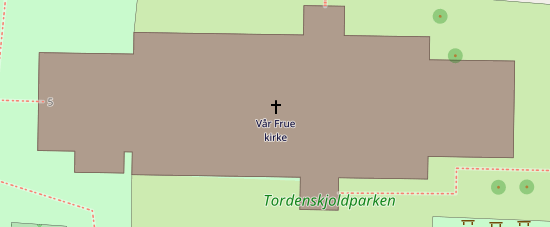
\includegraphics[scale=0.5]{figures/FixedByMe/fruekirke2D.png}
    \caption{2D representation of \textit{Vaar frues kirke}, result of listing \ref{eq:waytag1}. Source: openstreetmap.org}
    \label{fig:fruekirke2D}
\end{figure}

A relation is an ordered list of one or more nodes, ways, and/or relations and is used to define logical or geographical relationships between the other elements \cite{OpenStreetMape}. If a building consists of multiple parts, tagged with building:part=*, a relation is used to define the geographical relationship between the parts. Specifying roles to different parts is possible. A road can have role as east, going towards east. In multi-polygons, parts can have an inner or outer role, to specify whether it forms the inner or outer part of the polygon. A building relation is shown in listing \ref{eq:reltag}. There are eight members in this relation. The first member is a way, and it has an outline role creating the building footprint, for 2D representation. Listing \ref{eq:waytag1} is the XML-code for this way (notice that the ref number are equal to the way id in listing \ref{eq:waytag1}). The only node member in the relation contains the church's address. The rest of the members creates the 3D representation of the building shown in figure \ref{fig:fruekirke}.

\lstset{
    language=XML,
    morekeywords={encoding, relation, way, tag, node, member},
    label=eq:reltag,
    caption=Example of a relation tag - creating 3D representation of a church
}
\begin{lstlisting}
 <relation id="6269954" visible="true" version="2" changeset="39708156" 
  timestamp="2016-06-01T11:14:18Z" user="Peter Bremer" uid="366321">
  <member type="way" ref="89340594" role="outline"/>
  <member type="node" ref="2957446972" role=""/>
  <member type="way" ref="421821942" role=""/>
  <member type="way" ref="421821938" role=""/>
  <member type="way" ref="421821939" role=""/>
  <member type="way" ref="421821940" role=""/>
  <member type="way" ref="421821937" role=""/>
  <member type="way" ref="421821941" role=""/>
  <tag k="name" v="Vår Frue kirke"/>
  <tag k="type" v="building"/>
 </relation>
\end{lstlisting}

\begin{figure}[H]
    \centering
    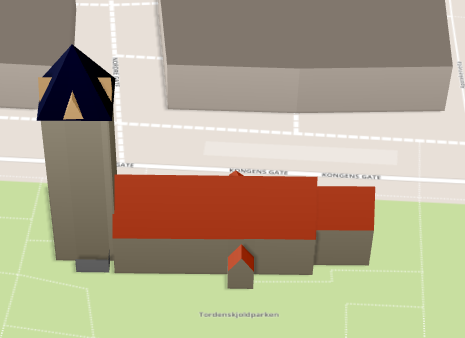
\includegraphics[scale=0.5]{figures/FixedByMe/fruekirke.png}
    \caption{3D representation of \textit{Vaar frues kirke}, result of listing \ref{eq:reltag}. Source: osmbuildings.org}
    \label{fig:fruekirke}
\end{figure}


 \section{Mapping buildings in OSM}\label{buildOSM}
A building can be represented by nodes, ways or relations in OpenStreetMap. When importing buildings into OSM, the XML-code representing the building must be tagged with Building=*. Frequent occurring values are house, residential and garage, describing the buildings particular usage.  Using the building tag in node representations is tolerated but not recommended. A building is much better expressed by their footprint (close way or multi-polygon), and if the footprint is available, one should not add the building key in nodes. The building key should be used to mark the buildings footprint. The most common occurring value for the building key is yes and used when it's not possible to determine a more accurate value \cite{OpenStreetMapf}. A list of possible values that can be added to the building key is listed on the OSM building wiki page. It is possible to introduce new values, but it is not recommended. The building key is most common used in way representations \cite{TagInfo2016}. An example of how to use building key in a way-tag see listing \ref{eq:waytag1}.

A building can also be represented by a relation. Relations are used if the building consists of multiple parts which physical differ from each other, often when a 3D representation of the building is created. A building relation mainly consists of two or more ways. A way then represents a part of the building and should be tagged with a building:part key and usually the value yes. Then the way-tags representing the different building parts are ordered together inside the relation. An example of a building:part=yes implementation can be seen in listing \ref{eq:waytag}. Note that the first and last <nd> tag refers to the same node, so this is a closed way. The key roof:shape with value gable gives the appearance of the roof. The result from the code in listing \ref{eq:waytag} is shown in figure \ref{fig:erkeinng} marked with a red line. A relation containing building:parts are shown in listing \ref{eq:reltag}. Notice that this relation is tagged with the key type and the value building. If a relation is tagged with type=building, it groups both building footprint and all building parts together. See figure \ref{fig:fruekirke} for a 3D building representation created with building parts. 

\lstset{
    language=XML,
    morekeywords={encoding,way, tag, nd},
    label=eq:waytag,
    caption=Example of a way tag - creating 3D representation of a building part
}
\begin{lstlisting}
  <way id="17533469" visible="true" version="22" changeset="39301425" 
  timestamp="2016-05-13T21:20:04Z" user="Peter Bremer" uid="366321">
  <nd ref="3505716655"/>
  <nd ref="2517225923"/>
  <nd ref="4184346715"/>
  <nd ref="3505716656"/>
  <nd ref="4184346713"/>
  <nd ref="4184346717"/>
  <nd ref="3505716654"/>
  <nd ref="4184346719"/>
  <nd ref="3505716655"/>
  <tag k="building:colour" v="#c3c0b9"/>
  <tag k="building:material" v="stone"/>
  <tag k="building:part" v="yes"/>
  <tag k="height" v="11"/>
  <tag k="name" v="Sydkapell"/>
  <tag k="roof:height" v="4"/>
  <tag k="roof:material" v="copper"/>
  <tag k="roof:orientation" v="across"/>
  <tag k="roof:shape" v="gabled"/>
 </way>
\end{lstlisting}

\begin{figure}[H]
    \centering
    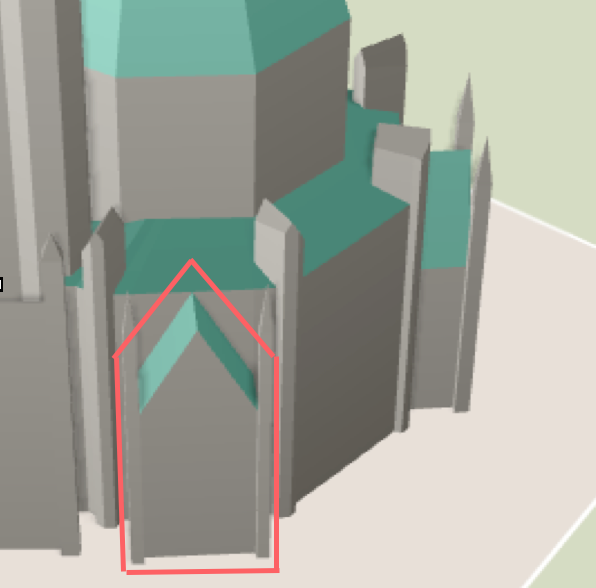
\includegraphics[scale=0.5]{figures/FixedByMe/nidaros3D.png}
    \caption{\textit{Sydkapell} with gabled shaped roof, result of listing \ref{eq:waytag}. \textit{Source: osmbuildings.org}}
    \label{fig:erkeinng}
\end{figure} 
%Microtasking chapter
\chapter{SOSI and FKB building}
This paper will look at FKB buildings and how it can be imported into OpenStreetMap. The FKB dataset comes in SOSI format. But what is SOSI? This chapter will give an introduction to SOSI, both standard, and format. The standard was developed by the Norwegian mapping authority and is the largest national standard for geographic information, where the standard is implemented in the SOSI format. SOSI is a widely used file format for Norwegian mapping \cite{Kartverketa}. FKB is a collection of datasets containing detailed vector data of Norway, created in the SOSI format. Since this paper looks at FKB building dataset this chapter will also describe FKB and the most common and valuable features for OpenStreetMap within the building dataset. Some features will not be relevant for import into OpenStreetMap. The chapter ends with an evaluation of SOSI, looking at its advantages against OpenStreetMap XML format.  

\section{SOSI}
The national standard for geodata in Norway is called SOSI, created by the Norwegian mapping authority. Geodata is map data stored in a digital format so that we can produce maps from it. The standard is based on international standards, primarily the NS-EN ISO19100-family of standards \cite{Skogseth2014}. The SOSI standard is implemented in the SOSI format, a Norwegian geospatial vector data format. The SOSI data consists of point -, line (\textit{kurve}) - and area (\textit{flate}) features. A point feature is only one single vertex, given in north and east coordinates with or without the height. Line feature is two or more vertices, but the first and last vertex are not equal. An area feature is three or more vertices, where the first and last vertex are equal. 

The Norwegian map authority has established a general feature directory \textit{(objekt katalog)} in connection with the SOSI standard. The purpose of a feature directory is to specify feature types and associated properties that are general within a discipline or across multiple disciplines \cite{Kartverket2016}.  The directory covers around 50 disciplines (2014) \cite{Skogseth2014}.  In SOSI version 4 the modeling method was changed, from modeling point, line and area to modeling feature types in the real world (buildings, roads, boundaries etc.) \cite{Skogseth2014}. For instance, a road will have many associated properties, in addition, it can be located as a line, this is how SOSI version 4 models its data.* %TERJE SKOG: Er dette riktig? Hva mener egt med at de endret metode? 

SOSI data can be presented on four different levels, each level represents a different data quality. %Level 1 is the simplest form, representing the data with feature type  x, y and H, no further properties. 
A SOSI dataset contains information on three levels. First are the \textit{Head} containing shared information about the dataset, this information applies to all data. Then comes the \textit{Data itself} containing properties and location coordinates (N, E and height). The SOSI dataset is finished with an \textit{End} which is the end of the data series \cite{Skogseth2014}.  

\section{FKB and data quality}

FKB, \textit{Felles Kartdatabase} in Norwegian, is a collection of structured datasets that contains the most detailed vector data of Norway. FKB data is collected through a collaboration called Geovekst. This is a collaboration between the Norwegian mapping authority, the Norwegian road authority, Telenor, Energy Norway, the Norwegian Association of Local and Regional Authorities, the ministry of Agriculture and the Norwegian Water Resources and Energy Directorate. \cite{Kartverketc}. FKB data comes as vector data in SOSI format \cite{Kartverket2011}. 

The FKB standard describes which features that is included in the mapping and the accuracy of the objects. There are specified four FKB standards, FKB-A, FKB-B, FKB-C and FKB-D \cite{Kartverket2011}. FKB-A is the most detailed, containing good three-dimensional data description and has high standards on accuracy (5-20 cm) and content. Most commonly used in city centers. FKB-B is also detailed with an accuracy of 20 - 30 cm. Most commonly used in urban areas. FKB-C is used for overview planning and management (\textit{forvaltning}) with an accuracy of 0.50 - 2.00 m. FKB-D are areas not covered by the three other standards, like mountain areas, and has a broad accuracy of 5 - 100 m. %The feature types in the FKB standard are divided into four classes, specifying the localization accuracy (the standard deviation).
Today, maps should always be produced after the FKB standards \cite{Skogseth2014}.

This paper will look into the FBK building dataset. The data consist of both point, line and area and contains 24 different feature types \cite{Kartverket2013}. The data is established and kept up to date by using photogrammetry. In some cases, the data is * %GRAMMAR: is eller are?
established by using land surveying \cite{Kartverket2013a}. Building points are transferred from the cadastre (\textit{Matrikkelen}). Data is* %GRAMMAR: is eller are?
 delivered in the official reference system for each municipality since the data are distributed per* %Kan man si per paa eng?
  municipality. 
  
Today FKB data is saved piecewise within each municipality. The data is collected in a database at the Norwegian mapping authority which is only updated one or two times a year. This is not the optimal solution. A goal is to gather all FKB data, from every municipality, into one central database where all updates will be made directly to this central database. The goal is to have 80\% of Norwegian municipalities connected to the database within 2018 \cite{Kartverket2016a}.  

Possibilities for 3D representation of buildings from the FKB standard varies. Some feature types in the FKB dataset have a level of detail attribute called \textit{TREDNIVÅ} where they usually use six levels. At level 0 solely 2D is supported, limited to the ground floor. In level 1, buildings are represented as blocks with a flat roof. The height of the roof is either the minimum, maximum or average of ceiling height around the building. Recognizability is not great. In level 2 the main shape of the roof is maintained with the use of ridge lines and break lines. Photogrammetric data capture for FKB-A, -B and -C standards provides buildings with level of detail similar level 2. Level 3 includes added features as dormers, balconies, larger chimneys etc. %A minimum size is introduced each feature type for details*. 
Gives a better visual quality and a more appropriate basis for analyses.  Photogrammetric data capture for FKB-A and -B standards provides a level of detail similar level 3, but details are different for the two standards. Level 4 is a high-quality model of buildings, not supported in the SOSI standard building model \cite{Kartverket}. Level 5 is a high-quality model of a building both outside and inside, not supported in the SOSI standard building model \cite{Kartverket}. FKB-A and FKB-B features describing the main roof has to be at least level 2 of detail and features describing details located at the roof with at least level 3 of detail. 

\section{Features in FKB building}\label{sec:FKBbuilding}
% P = påkrevd (obj. typen skal være med i FKB)
% B = betinget (obj. typen skal være med under bestemte bet.)
% O = opsjon (det må spesifiseres i det enkelte prosjekt om objekttypen skal inngå)
% Er en god del, de som er relevante for OSM . Viktigste obj typene for OSM. Backe opp med 3D 
Looking at a FKB building dataset covering Trondheim municipality gives some indication of the most common feature types and help to determine which features should be prioritized in the conversion between FKB building SOSI format and OSM file format. This section will use the Trondheim municipality dataset. The dataset contains 1499 point objects, 618 710 line objects and 95 071 area objects. This municipality has a fairly large city center and a good variation in building types. %like apartment buildings, separate houses (\textit{eneboliger}) and terrace house (\textit{rekkehus}). 
Therefore this dataset is a good representative of the average municipality in Norway. 

There are 24 different feature types in the FKB building dataset. Where two features are point data,  three features are area  (\textit{flate}) data and the rest is line (\textit{kurve}) data.  The features are grouped into four categories, building and building refinement (\textit{bygningsavgrensning}), descriptive building lines, building appendage (\textit{bygningsvedheng}) and lastly roof covering (\textit{takoverbygg}). 

\begin{figure}[H]
    \centering
    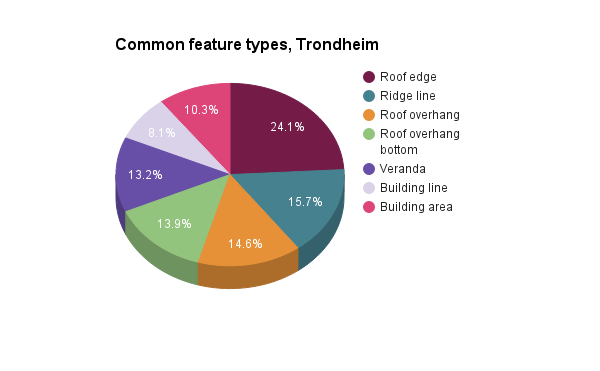
\includegraphics[scale=0.5]{figures/FixedByMe/comm_feature_type.png}
    \caption{Most common feature types in Trondheim}
    \label{fig:commfeattypes}
\end{figure} 

When considering an import to OpenStreetMap there will be features that are not as relevant. Adding all buildings as point data does not seem relevant. The two feature types within point data are building and assistantpoint3D (\textit{hjelpepunkt3D}). The building feature comes as both point and area, containing exactly the same attributes. If the building footprint is available, points should not be imported, as mentioned in section \ref{buildOSM}.  Therefore, the building feature as point data should not be imported into OSM, it will not add additional information. The assistantpoint3D will not be imported when excluding the building point feature. Conclusion is that no point data will be relevant for import.* %Rewrite?

%Starting with line data, which in the FKB dataset covering Trondheim consist of 618 710 rows. 
In Trondheim there are 158 917 roof edge (\textit{takkant}) features and is the most common line feature in this municipality. This feature is the building's exterior roof surface refinement (\textit{avgrensning}). See figure \ref{fig:kurve_tak_fkb} and \ref{fig:kurve_4tak_fkb} for examples on where this feature is mapped on buildings. The second most common line feature is ridge line (\textit{Monelinje}). There are 103 488 objects with this feature in Trondheim. Ridgeline is the line describing the horizontal bending line / break line (\textit{knekklinje}) on top of the roof and is also the highest peak of the roof. See figure \ref{fig:kurve_tak_fkb} and \ref{fig:kurve_4tak_fkb} for example of where it is mapped on buildings. A minimum goal for the FKB mapping team is to map ridge lines on every building \cite{Kartverket2013a} and can explain the hight frequency of this feature \cite{Kartverket2013a}. 

\begin{figure}[H]
    \centering
    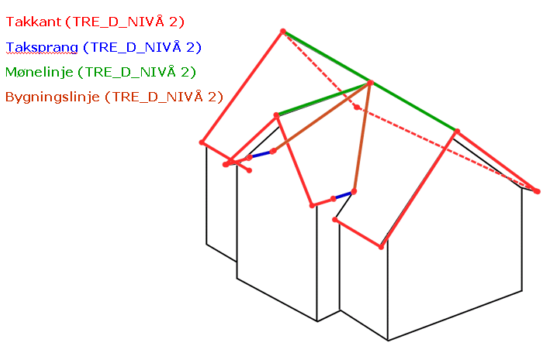
\includegraphics[scale=0.5]{figures/kurve_4tak_fkb.png}
    \caption{Roof edge (red), roof overhang (blue), ridge line (green) and building line (brown) \cite{Kartverket2013a}}
    \label{fig:kurve_tak_fkb}
\end{figure} 

Third most common line feature in Trondheim is roof overhang (\textit{taksprang}) with 96 436 objects. This feature describes the top of the roof edge inside the building shell, not located on the outside edge which is the roof edge feature. For an example see figure \ref{fig:kurve_tak_fkb} and \ref{fig:kurve_4tak_fkb}. This feature should be mapped where height difference between two roof levels is larger than the tolerance of the FKB-data. This feature is in the descriptive building lines category. The line always follows the roof edge. 

\begin{figure}[H]
    \centering
    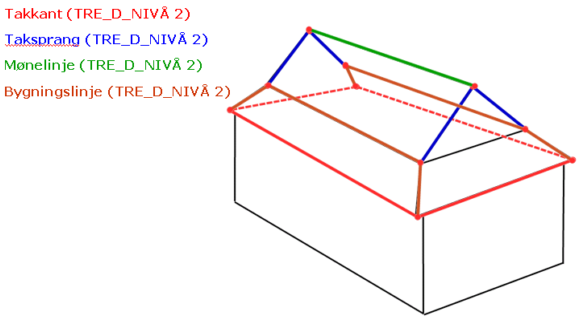
\includegraphics[scale=0.5]{figures/kurve_4tak_fkb2.png}
    \caption{Roof edge (red), roof overhang (blue), ridge line (green) and building line (brown) \cite{Kartverket2013a}}
    \label{fig:kurve_4tak_fkb}
\end{figure} 

Fourth most common line feature in Trondheim is roof overhang bottom (\textit{TakSprangBunn}) with 91 281 rows. This feature describes lines located at the bottom of a roof edge within a building mass (\textit{bygningskropp}). Roof overhang bottom is under the descriptive building lines category. In figure \ref{fig:taksprangbunn} the blue line shows where a roof overhang bottom line can be drawn. As shown in figure \ref{fig:taksprangbunn} roof overhang bottom lines should, if possible, have equal coordinate values (N, E) as the corresponding roof overhang. This is visualized with the dashed black lines on figure \ref{fig:taksprangbunn}. In figure\ref{fig:taksprangbunn} the red and blue lines are from the original figure in \cite{Kartverket2013a}, the green line is added afterwards to visualize roof overhang in the same figure.  

\begin{figure}[H]
    \centering
    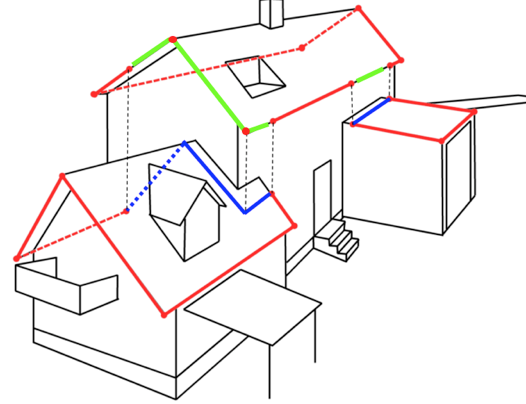
\includegraphics[scale=0.4]{figures/FixedByMe/kurve_3fkb_tak.png}
    \caption{Roof overhang bottom (blue), roof edge (red) and roof overhang (green)}
    \label{fig:taksprangbunn}
\end{figure} 

Fifth most common line feature in Trondheim is veranda and includes veranda, terrace, balcony and loading ramp \cite{Kartverketb}. If the area mapped is following FKB-A standard veranda features down to 2 square meters are drawn, and down to 6 square meters if the area is following FKB-B standard. Veranda features have an attribute value MEDIUM that describes if it is located on the roof (MEDIUM = B), on the outer wall (MEDIUM = L) or on terrain (MEDIUM = T). This attribute is helpful when making 3D models of the buildings. Height attributes can either be a reference at the top of the railing (used for medium B) or at floor level (used for medium T). When the feature has attribute medium L its optional which height reference to use. See figure \ref{fig:veranda} for example of veranda features. Veranda features are under the building appendage category. 

\begin{figure}[H]
    \centering
    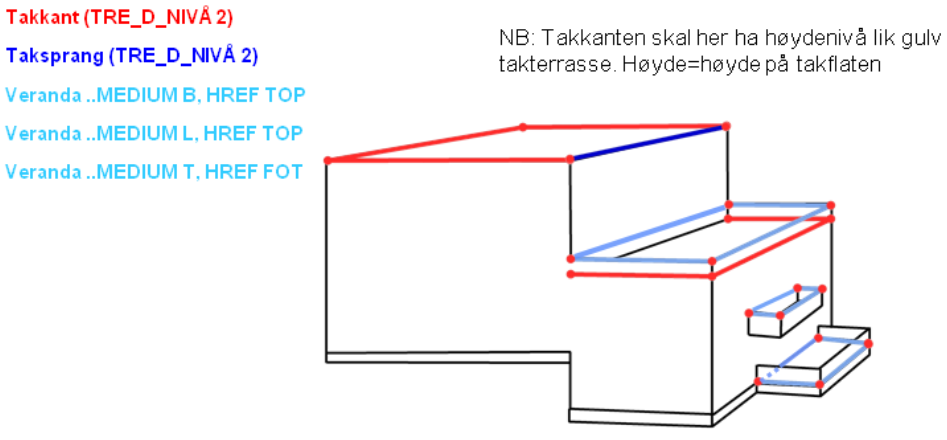
\includegraphics[scale=0.4]{figures/veranda_fkb.png}
    \caption{Roof edge (red), roof overhang (blue) and veranda (turquoise) \cite{Kartverket2013a}}
    \label{fig:veranda}
\end{figure} 

Sixth most common line feature in Trondheim is building line (\textit{bygningslinje}) with 53 255 rows. The feature describes building details which are within a roof perimeter, and which cannot be described by other feature types. If data covering the area is within the FKB-A standard %TERJE: Hvordan formulere dette best?
the building lines should be drawn on objects that are 2 cubic meters or larger and if it's within the FKB-B standard only objects that are 7.5 cubic meters or bigger should be drawn. The two limits are just instructive, some interpretations will be done. Examples of use can be seen on figure \ref{fig:kurve_tak_fkb} and \ref{fig:kurve_4tak_fkb}. 

Most important area feature is building, the two other features are otherBuilding and RoofCovering/RoofSuperstructure, like a carport. There are three types of building demarcation (\textit{bygningsavgrensning}) defined in FKB, foundation wall outline (\textit{grunnmurriss}), facade outline (\textit{fasaderiss}) and roof outline (\textit{takriss}. If more than one of them exist, roof outline will form the surface of the building feature. Building feature has an type of building attribute, which is an initial value mapped to a specific building type. House (\textit{enebolig}) has initial value 111 and dormitory (\textit{studenthjem}) value 152 \cite{Kartverketd}. Height reference is either measured from top, bottom or is unknown. 

It is impossible, at least in FKB, to create a specification of registration of buildings that are completely accurate. The buildings will always be subject to some generalization. This can be seen in the figures used in this section. 

\section{Benefits using SOSI in context of OSM}\label{sec:sosiosm}
%Ikke har et poligon direkte, flate er bare referanse til linjene Point, line, area (flate)

Listing \ref{eq:arebuild} is SOSI code for area representation of a building. FLATE means area and contains the feature id. OBJTYPE is feature type and in listing \ref{eq:arebuild} equals building, representing what the key would be in OSM. KOMM field contains a municipality code, representing the buildings municipality. BYGGNR is the buildings unique number found in the cadastre. BYGGTYP NBR is the description of what the building actually is used as or approved as. For instance in listing \ref{eq:arebuild} BYGGTYP NBR equals 182, meaning this building is a garage attached to a holiday home (\textit{fritidsbolig}) \cite{SOSI-sekretariatet}. This attribute will give the value to the building key in the mapping to OSM. BYGGSTAT is the building status where value TB means that the building is being used. 

Area representations in SOSI can refer to other geometry types. This is similar to how way and relation representations can refer to other objects in OSM. The REF field refers to the other geometry features using the feature id for the object being referred to. In listing \ref{eq:arebuild} REF equals -166775, which refers to the line feature in listing \ref{eq:linebulpart}. The minus sign in REF's value means that it refers to the line in listing \ref{eq:linebulpart} but with opposite direction. 

\lstset{
	language=XML,
	morekeywords={encoding,way, tag, nd},
	label=eq:arebuild,
	caption=Example of a area representation of a building in SOSI
}
\begin{lstlisting}
  .FLATE 715280:
..OBJTYPE Bygning
..KOMM 1601
..BYGGNR 196122907
..BYGGTYP_NBR 182
..BYGGSTAT TB
..KOPIDATA
...OMRÅDEID 1601
...ORIGINALDATAVERT "Trondheim kommune"
...KOPIDATO 20160502
..REF :-166775
..NØ
703226400 55444400
\end{lstlisting}

Listing \ref{eq:linebulpart} is a line representation of a building part. Here the feature type is roof edge, examples of a roof edge is shown in figure \ref{fig:kurve_tak_fkb} and \ref{fig:kurve_4tak_fkb}. OSM XML code of the same roof edge is shown in listing \ref{eq:roofedge}. Both listings refer to 6 different point representations. In listing \ref{eq:linebulpart} the point coordinates are written directly in the representation. NØH is north, east and height value for each point. KP1 means that this point is a connection point, but this is not implemented in the OSM XML code. In listing \ref{eq:roofedgexml} the XML codes refers to 6 different nodes (first and last node are the same). This is not possible in line representation through SOSI format. Only area representation can refer to other geometry features \cite{Kartverket2006}. This is one major difference between SOSI format and OSM XML format. 

\lstset{
	language=XML,
	morekeywords={encoding,way, tag, nd},
	label=eq:linebulpart,
	caption=Example of a line representation of a building part in SOSI
}
\begin{lstlisting}
.KURVE 166775:
..OBJTYPE Takkant
..DATAFANGSTDATO 20100610
..VERIFISERINGSDATO 20150627
..REGISTRERINGSVERSJON "FKB" "4.01"
..KVALITET 24 19 0 24 23
..TRE_D_NIVÅ 2
..KOPIDATA
...OMRÅDEID 1601
...ORIGINALDATAVERT "Trondheim kommune"
...KOPIDATO 20160502
..NØH
703226612 55444485 1344 ...KP 1
..NØH
703226525 55444618 1280
703226160 55444380 1280
703226247 55444247 1344 ...KP 1
..NØH
703226328 55444123 1283
703226693 55444361 1280
703226612 55444485 1344 ...KP 1
\end{lstlisting}
 

\lstset{
	language=XML,
	morekeywords={encoding,way, tag, nd, node},
	label=eq:roofedgexml,
	caption=Example of a line representation of a building part in OSM XML
}
\begin{lstlisting}
<way id="-166775" version="1" visible="true">
	<tag k="KOPIDATO" v="20160502"/>
	<tag k="OMRÅDEID" v="1601"/>
	<tag k="KVALITET" v="24; 19; 0; 24; 23"/>
	<tag k="TRE_D_NIVÅ" v="2"/>
	<tag k="ORIGINALDATAVERT" v="Trondheim kommune"/>
	<tag k="REGISTRERINGSVERSJON" v="FKB; 4.01"/>
	<tag k="OBJTYPE" v="Takkant"/>
	<tag k="VERIFISERINGSDATO" v="20150627"/>
	<tag k="DATAFANGSTDATO" v="20100610"/>
	<tag k="KURVE" v="166775"/>
	<nd ref="-161600" />
	<nd ref="-387568" />
	<nd ref="-387569" />
	<nd ref="-387570" />
	<nd ref="-387571" />
	<nd ref="-387572" />
	<nd ref="-161600" />
</way>
\end{lstlisting}

Listing \ref{eq:xmlnode} is the point features the way XML code listing \ref{eq:roofedgexml} refers to. 

\lstset{
	language=XML,
	morekeywords={encoding,way, tag, nd, node},
	label=eq:xmlnode,
	caption=Example of a line representation of a building part in OSM XML
}
\begin{lstlisting}
	<node id="-161600" lat="63.4147679" lon="10.0904069" 
		version="1" visible="true"/>
	<node id="-387568" lat="63.4147599" lon="10.0904333" 
		version="1" visible="true"/>
	<node id="-387569" lat="63.4147275" lon="10.0903844" 
		version="1" visible="true"/>
	<node id="-387570" lat="63.4147355" lon="10.0903580" 
		version="1" visible="true"/>
	<node id="-387571" lat="63.4147430" lon="10.0903335" 
		version="1" visible="true"/>
	<node id="-387572" lat="63.4147754" lon="10.0903824" 
		version="1" visible="true"/>
\end{lstlisting}

The roof edge represented by listing \ref{eq:roofedgexml} is shown in figure \ref{fig:roofedgeeks} where the numbers represent the drawing order. The point marked with 1 is \textit{<nd ref="-161600"/>} and the point marked with 6 is \textit{<nd ref="-387572" />}. 

\begin{figure}[H]
    \centering
    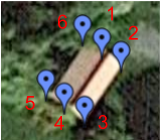
\includegraphics[scale=0.9]{figures/FixedByMe/sosiArea.png}
    \caption{Roof edge representation}
    \label{fig:roofedgeeks}
\end{figure} 


There are multiple similarities between the SOSI format and OSM XML format as shown in this section. Neither SOSI or OSM has a polygon representation directly and both have open and closed line representations. Feature types in SOSI are easily mapped over to key-value relations in OSM. FKB's way of representing buildings is also benefitial when modeling building parts in OSM, especially in 3D modeling. FKB contains line representation of every building part. This is why a SOSI to OSM converter is beneficial instead of a shape to OSM converter for instance.* %Bør jeg forklare mer eller kanskje ta noen av poengene med ned til siste kapittel?


\chapter{Micro-tasking}\label{ch:microtask}
To be able to import FKB building data into OpenStreetMap an import method is desired. A promising method is micro-tasking. This chapter will give an introduction to what the micro-tasking method is. It will describe what micro-tasking is and introduce related tools using this method. 

\section{Micro-tasking method}
The simplest type of tasks are called micro-tasks and should be accomplished from a few minutes to a few hours. The tasks are simple tasks, often highly repetitive. Tasks are often grouped together into one project or a campaign. In Non-profit organizations, it can be hard to get enough people involved, especially if it requires a lot of time from the volunteers. Micro-volunteering helps people volunteer without demanding all their time. The volunteers are only required to work in a limited time completing as many micro-tasks as their available time allows. When using the OSM Tasking Manager on mapping projects volunteers can complete mapping tasks within a reasonable time interval. This is a good solution for getting more volunteers to contribute who struggle to fit the volunteer work into their busy schedules. This concept has a huge potential but lacks awareness \cite{Bernstein}. The term micro-volunteering appears from the Spanish organization "Microvoluntarios", an online platform which allowed charities to post micro-tasks and connect to volunteers who can perform the tasks \cite{Madalena}.  Strengths of using micro-tasks are, among others, flexibility and convenience for the mappers \cite{Madalena}. Jim McAndrew said in his NYC state of the map US 2015 speak that micro-tasking can benefit OpenStreetMap and gives a lot of opportunities to the community, micro-tasking is the way of the future \cite{McAndrew2015}.  

\section{OSM Tasking Manager}
Micro-tasking in OpenStreetMap is done through, among others, the OSM Tasking Manager tool. The purpose of the OSM Tasking Manager is to divide a mapping job into smaller tasks. The tool improves project awareness since information about the project and tasks is very easily accessible. The interface present the user with an overview of which areas needs to be mapped and which areas needs validation. It has an overview of how much work is left, how much is finished and general information about the mapping and introductions on how to do it. A common mapping project can be to map every building in an area using aerial photos. The area is divided into equal grids and displays different color codes. Yellow means that this grid is being mapped by someone else, red means that the area is marked as finished but are waiting for validation by another user and green indicates that this area has been inspected in the OSM database for completeness and compliance \cite{Palen2015}. Empty grids mean that the area covered needs mapping. An example of a project in the OSM Tasking Manager is shown in figure \ref{fig:project2261}. The project aims at mapping road networks, residential areas and buildings in the area marked \cite{HOTTaskingManager2016}.  

\begin{figure}[H]
    \centering
    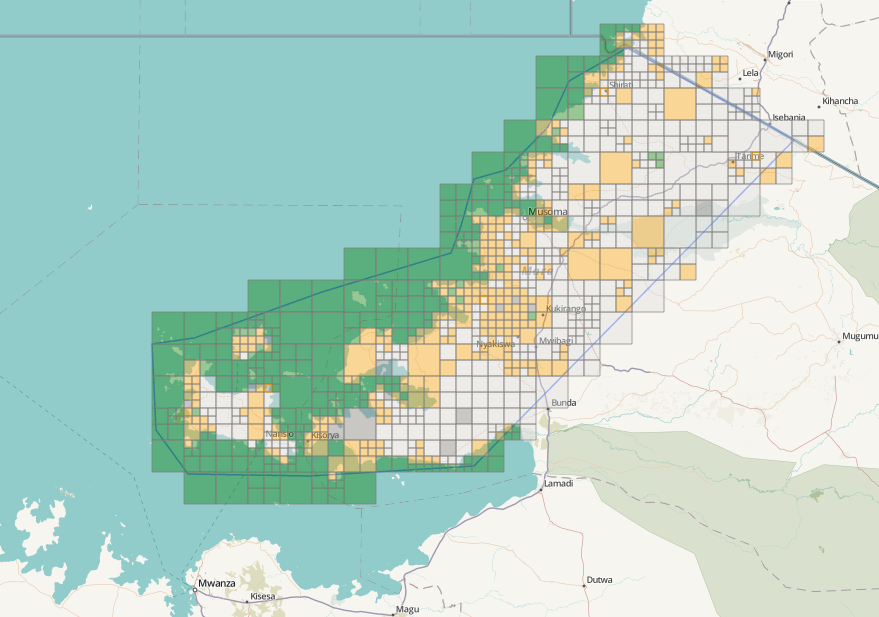
\includegraphics[scale=0.3]{figures/FixedByMe/taskingmanager.png}
    \caption{Project 2261- Tanzania Development, source: tasks.hotosm.org}
    \label{fig:project2261}
\end{figure} 

The OSM Tasking Manager has in the aftermath developed to other projects outside the HOT community. Especially import projects have had good leverage in this tool, more about this in chapter \ref{ch:importmethods}. Newer versions of this tool gave mappers the possibility to asynchronous communicate on tasks, making it easier to inform each other. Unfinished tasks often contain information from users who have been working on it with an explanation of what they mapped or what they didn't map. The Los Angeles building import, which started in 2015, developed the OSM Tasking Manager 2, adding new features to fit their needs. Adding possibilities for tasks being polygons and not grids. 

\begin{figure}[H]
    \centering
    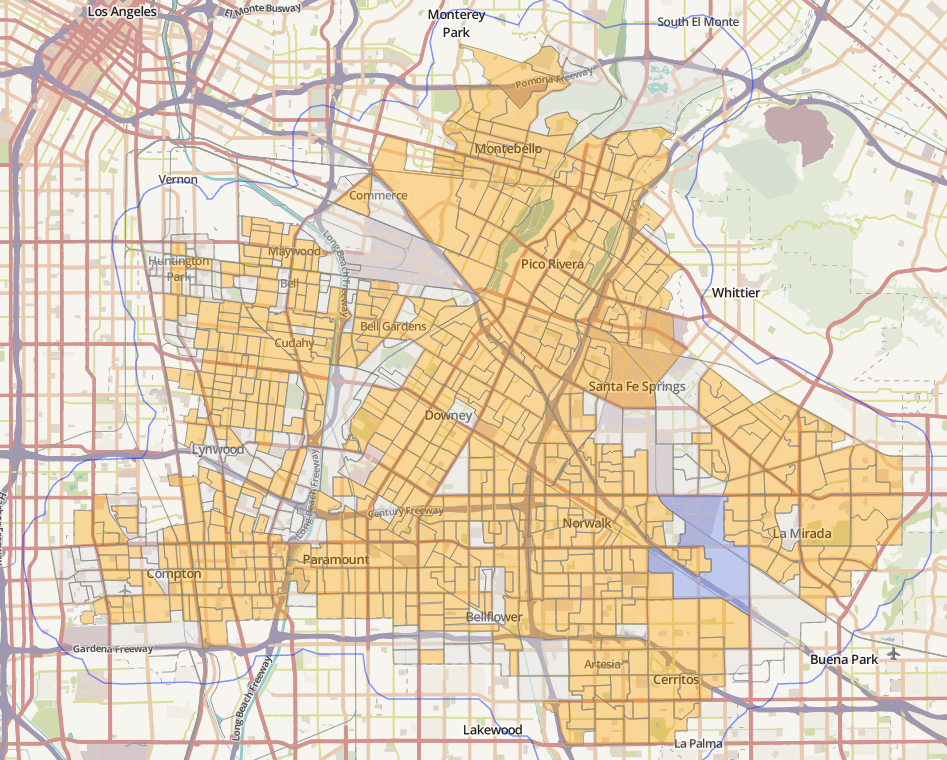
\includegraphics[scale=0.3]{figures/FixedByMe/taskingman2.png}
    \caption{Project 2 0- Southeast - LABuildings Import, source: labuildingsimport.com}
    \label{fig:project20}
\end{figure} 

An example of the OSM Tasking Manager 2 used by the Los Angeles building import team is shown in figure \ref{fig:project20}. Notice that instead of grids they use polygons, dividing the tasks into a reasonable size using census block groups. More about this in subsection \ref{sec:importmicro}. 

\section{Other tools}
%To-fix, map-roulette 
Other tools in OSM that also use the micro-tasking method are often designed for fixing bugs in the OSM database. Both Map-roulette and To-fix are examples of such tools and are listed as error detection tools on the OSM quality assurance wiki page. MapRoulette was created by Martijn van Exel and Serge Wroclawski, and its slogan is "\textit{Towards a better map, one bug at a time}." This tool has a gamified approach to fixing bugs, breaking common OSM data problems into micro-tasks. According to its founder Martijn, MapRoulette has become a very popular mapping pastime for both amateur contributors and experienced mappers \cite{Exelvan2013}.  The tool breaks tasks that need fixing into challenges with a tutorial on how to best fix the issues in the challenge. It displays one issue at a time, once every issue in a task is fixed a new challenge is activated. Common issues are connectivity errors among ways, overlapping ways and equivalent ways \cite{OpenStreetMapk}. To-fix is a micro-tasking tool creates by MapBox and is very similar to MapRoulette. This tool breaks up large mapping jobs into smaller tasks that multiple people can work on asynchronously \cite{Lidman2014}. The tasks are queued up, then a group of mappers can do the tasks and track their progress. Tasks presented here are also commonly fixing overlapping and crossing highways. With To-fix, issues can be fixed through the iD editor or JOSM editor. This tool do not give an introduction to the tasks like MapRoulette, making it more challenging knowing what to do. To-fix loads tasks much faster then MapRoulette who are quite slow. There are also bugs in MapRoulette. For instance, half of the information text are not displayed because it's too long for the information box and the skip button do not work properly. Both solutions convey statistics presenting total fixed, skipped and marked as not error on tasks. 
 \chapter{OSM import methods}\label{ch:importmethods}
%1. Helautomatisk, scriptet import \\
%2. Helmanuell import basert p  tracing av f.eks WMS-data\\
%3. Guidet automatisk import (slik import av n50-data blir gjort i OSM i dag) \\
%4. Import basert p  metodikken LA-buildings-prosjektet har gjort, og som beskrives av McAndrews (microtasking)

%Conflation \href{http://wiki.openstreetmap.org/wiki/Conflation}{Wiki Conflation}
The traditional way to contribute data to the OpenStreetMap project is through active users who use their GPS to track roads and their local knowledge to add information about geographic regions to the OSM database \cite{Zielstra2013}. Users also digitalize aerial photos by drawing buildings etc. from it. Cheaper GPS receivers and more available satellite imagery with better resolution make it easier for users to contribute \cite{Chilton}. The number of active users in different regions varies, making some regions on the OSM map full of data while others are almost empty. The varying number of active mappers led to a second approach for getting data into the OpenStreetMap database; bulk imports \cite{Zielstra2013}.  Bulk import is the process of uploading external data and was meant for initial/preliminary object class uploads, so only if the object were none existing in the area  \cite{Zielstra2013}.  It's a good alternative for countries or regions with few or none active users. Through the years different import methods have been developed. This chapter will evaluate the three common import methods. A fully automatic method, a guided automatic method and the micro-tasking method. %This will hopefully give a good indication if the micro-tasking method can be a suited import method. 

\section{Fully automatic import script}
Creating a script that automatically imports big datasets into OpenStreetMap, a bulk import, is not encouraged in the OSM community \cite{Zielstra2013}. This becomes clear when reading the wiki pages about import. A bulk import is supposed to be a supplement to user generated data. The user-generated data and the user's ability to work is always the priority \cite{OSMimport}. A fully automatic import do automated edits to the OpenStreetMap database with little, if any, verification from a human. Automatic edits are changes that have no or very limited human oversight \cite{OSMAutiEdit}. This kind of edits must follow the Automated Edits code of conduct \cite{OSMAutomaticEdits}. The policy was created to prevent damaging acts on the database and ignoring it will result in the import be treated as vandalism. 

An example of a bulk import was the TIGER import. The Topologically Integrated Geographical Encoding and Reference system (TIGER) data was produced by the US Census Bureau and is a public domain data source. The bulk import was completed in early 2008 \cite{Zielstra2013}, populating the nearly empty map of the United States. The TIGER dataset was not perfect and had its faults, but it was better than no data at all \cite{Willis2008}. The import mainly focused on data containing the general road network of the US \cite{Zielstra2013}. 

Reading through the OpenStreetMap mailinglist called talk, it becomes apparent that this import is an automatic edit with very limite oversight. "\textit{Please don't upload Northampton County, [..] I've mapped my entire town there [..]}" \cite{Mielczarek2007}.  Active OSM mappers following the maillinglist are trying to save their manual work. Users not attending the mailing list had limited, if any, possibilities of saving their work through the TIGER import. Mappers importing TIGER data tried not to override existing data. They started on empty states but reading through the "TIGER, which states next?" mailing thread the decisions on which state to import next was solely based on the people attending the conversations. \textit{"I believe I'm the only one out here in Nebraska [..] Feel free to override my edits"} \cite{Bishop2007}. The import process did not have any requirements on what they should do with existing data. OSM mappers added the TIGER data county by county, state by state. The OSM user Dave Hansen, one of the most active users during this import, created a text file with his upload queue and published it on his dev openstreetmap site \cite{Hansen2007a}. He added states and counties after requests from users \cite{Hansen2007}\cite{Hansen2007b}. The import team did not have any validation or correction methods or routines. In the aftermath of the import, tagging errors of. For instance, the TIGER data groups residential, local neighborhood roads, rural roads and city streets into one road class, while OSM uses a more refined data schema with various highway tags for multiple road classes \cite{Zielstra2013}.

On the OSM TIGER wiki page, last updated August 2016, they say \textit{it is unlikely that the TIGER data ever will be imported again}. The main reason is the growing US mapping community, and their mapping is often better than the TIGER data. \textit{"Do not worry about getting your work overwritten by new TIGER data. Go map!"}  \cite{WikiOSMTIGER2007}. A new bulk import with updated TIGER data can overwrite existing, more precise data. The TIGER data are of variable quality, poor road alignment is a huge problem and also wrong highway classification. Many hours of volunteer work could just be lost, and this is something the community want to avoid. The bulk import in 2007 got the United States on the OSM-Map and saved the mapping community a lot of time finding road names etc. \textit{"TIGER is a skeleton on which we can build some much better maps"} \cite{Willis2007}. On the opposite side the project kept the US mappers away, they were told for years that their work was no longer needed after the TIGER upload was complete. But the presence of TIGER data ended up requiring a lot of volunteer help, fixing errors like the poor road alignments and wrong tagging. 

Bulk imports are overall not recommended today but have been helpful as well. In the Netherlands, bulk imports have met little resistance, mainly because the import work are done by dedicated OpenStreetMap mappers who know the OSM import guidelines.  Arguments for bulk imports say that a map that already contains some information is easier to work on and can help lower the entry barriers for new contributors. Another argument is that an almost complete map is more attractive for potential users, that again can encourage more use of OSM data in professional terms \cite{Exelvan2010}. But a huge minus to bulk imports is the data aging since the data being imported usually is a few years old and updating it takes time, often years. The TIGER import was data from 2005, but the import finished in 2008 \cite{Zielstra2013}. Between the time of first import and update, the community has fixed bugs, added necessary metadata, and the community would not want to lose that data/information. 

%Today there are huge amounts of object types in OpenStreetMap. Bulk imports with limited human interaction do often end up overriding existing data, which is one of the "don't do" points on the import guidelines list on the osm wiki page. OpenStreetMap do not have layers, so data on top of data makes it very difficult to find and organize the data.    
%has common errors like wrong road classifications, adds roads that no longer or never existed, railway and roads 
%moved so they intersect when they do not. 

%\section{Fully manually import based on tracing}
%This method can be very time-consuming. The mapping quality depends on the image resolution in the area beeing mapped, and it is also hard to add metadata from an image. For instance, it's impossible to see the height of a building from a satellite image. 

\section{Guided automatic import}\label{guidedautoimp}
Fully automatic import of huge amounts of data is discouraged in the OSM community, so another approach is guided automatic import. The OSM community encourages people to import only small amounts of data at a time and only after validation and correcting errors \cite{Mehus2014}. This method was applied when the OSM-community in Norway got approval from the Norwegian map authority to import N50 data \cite{Kihle2014}. N50 is the official topographic map of Norway, and provide a good data foundation. The import process is described on the OSM Topography import for Norway wiki page. The mapping team imported one municipality at a time. Each municipality dataset was divided up in .15 deg time .15 deg grid changesets, and each changeset contained from five thousand to twenty thousand elements \cite{OSMN502014}. The N50 import was a community import, but especially experienced user was encouraged to import the data \cite{Mehus2014}. 

The N50 release was good news for Norway, since regions, especially in northern parts of Norway, had limited amounts of data because of few active OSM mappers. This import would then increase the quality of OpenStreetMap in much bigger parts of Norway \cite{Jorgenrud2013}. It's a huge dataset, so they had to import it with caution, not everything in the dataset was relevant for OpenStreetMap, this is noted by the OSM user Solhagen \cite{Solhagen2015}. %Another approach is to convert the sosi files to shp through GDAL and import this shp file into JOSM. This approach is not recommended, converting sosi to shape will result in loosing important data.  SOSI uses a hierarchical metadata structure  

The OSM user tibnor preprocessed the data and uploaded to a google drive folder available for everyone. He started on the preprocessing early 2015. Late 2013 the OSM user gnonthgol* created sosi2osm script for conversion between SOSI format and OSM file format, which he informed about in the sosi2osm mail thread \ref{mail:nuugkart}. This script is the recommended way of converting the N50 SOSI files since it converts directly from SOSI to OSM XML format. In May 2015 tibnor released a JOSM plugin for the N50 import of rivers/streams to make it faster to check and fix directions. The import process was managed through a wiki page. Here users wrote their name and progression, start date and end date of the imported municipality. Elements which needed manual inspection or validation was tagged with "Fix-me" and a description of what to do. They used a python script ("replaceWithOsm.py") to merge N50 data with existing OSM data, adding source=Kartverket N50 tags on the new data. Elements that already exists in OSM, that conflicts with the new data, is marked with FIXME=Merge. Here the user has to search for the conflicting elements and correct the errors manually. Then the data can be uploaded to OSM. 

The N50 import was initially stopped in May 2014 by Paul Norman. The Norwegian OSM group started importing the N50 data before consulting with the OSM imports mailing list, which is required. They were also importing the data without the proper approach. The wrong import approach was pointed out by DWG member Paul Norman \cite{Mehus2014}.  DWG is the data working group, created in 2012, and they are authorized by the OSMF to detect and stop imports that are against the import guidelines \cite{OSMDWG}. The Data working group reverted the import because of technical problems and errors in the import \cite{Didriksen2014}. The reset was a step back for the Norwegian OSM team, and they had to start over again. The DWG stopping the import in 2014 was probably for the best. They have much experience with automated imports. 

The N50 import has been time-consuming. It started in 2015 and is still not finished, even though most of the municipalities are imported. The import process was carried out according to the import guidelines. Without the DWG group, the import would probably end up as an automated edit with no proper validation process. The N50 import is one example of how time-consuming this process can be. There are guidelines to follow, a lot of validations to be done. % importing existing data into OpenStreetMap is a time-consuming job. 

\section{Import based on micro-tasking}\label{sec:importmicro}
The N50 import was a good start towards micro-tasking an import of huge amounts of data. They divided every municipality into .15 degree .15 degree grid changesets and imported one changeset at a time. Both the New York building import finished in 2014, and Los Angeles building import, not finished, took this mindset to the next level, creating a Tasking Manager interface particular to this import, among other initiatives. The LA-building team created a custom tasking manager to coordinate the LA County building import \cite{OSMTaskingManager}, while the NY-team used the original OSM Tasking Manager. 

In the Guided automatic import from \ref{guidedautoimp} we saw that dividing datasets into smaller parts makes the import easier to, among others, distribute the workload between experienced users. OSM Tasking Manager takes this approach further by among others, offering a graphical user interface around the import. The tasking manager contains essential information. Like a description of the import, instructions on how to do the import and which tags to use, etc. It provides an easy way of downloading a dataset, bounded by a grid, into JOSM or id editor.

The New York building import took ten months, finishing in June 2014. The project started as a community import but underestimating the import complexity and time spent training and supporting new mappers they restarted a few months in, loosely forming a group around the project \cite{Barth2014}. The group consisted of volunteer mappers and employees from the Mapbox team. This grouping made coordination easier and also made it simpler to ensure proper training \cite{Barth2014a}. More than 20 people spent more than 1500 hours, importing 1 million buildings and over 900 000 addresses \cite{Barth2014}. Common issues during import were written on the Github page. The New York City data was first converted into OSM file format, then cut into byte sized blocks which were reviewed and imported manually through the tasking manager, piece by piece. An important validation step was that a different person than the original importer validated the data, reviewing it for errors and cleaning up when needed \cite{Barth2014}. 

The LA building import started in 2014. Two OSM enthusiasts started on the project, Jon Schleuss, and Omar Ureta. They used code from the NY building import and adapted it to their needs. After a while, Mapbox joined in on the import, an important step for the project. Mapbox helped with important programming, creating scripts, converting the data to osm files, creating block groups of the data. The first challenge was to decide which datasets to import.  They ended up neglecting address data, which would \textit{delay the project with 1 year or 2} - quote Jon Schleuss, adding just building outlines and building info (assessor data) \cite{Schleuss2016}. They merged and cleaned the datasets, splitting them into blocks and serving the data to the tasking manager. They used mapathons to get the import started. MaptimeLA was the organizer, and they also created tutorials for new mappers who joined the team. The first mapathons started with JOSM training to new mappers. Evolving to only arranging import mapathons, or import parties. Through mapathons is was easier for inexperienced mappers to contribute, here they could get the necessary training.  When importing data mappers always have to examine for possible conflicts between existing and new data. If a conflict is detected, and the mapper doesn't know how to deal with it, they can flag the .osm file, and a more advanced user will look at it. The task will then be finished by someone else. 
%Mapathon example https://www.meetup.com/MaptimeLA/events/233592014/

A big difference between the NY building import and LA building import was that the NY team ended up only allowing some OSM users to import. The NY-import was planned as a community import, but underestimating the import complexity and time spent training and supporting new mappers they restarted a few months in,  they loosely formed a group around the project \cite{Barth2014}. The LA building team allowed everyone to join the import. To keep track of mappers the LA team created a list where the volunteers had to write their import username \cite{Sambale2016s}. Doing the import job during mapathons is a good idea, making it easier to have an overall control over the import process. 

In NY building import, when an error was detected that required updates to already imported data they had to do an automated edit. Updating existing data manually was very time-consuming. Updating OpenStreetMap data programmatically, with a script, is according to Alex Barth in Mapbox, crucial for a successful import.  The LA community has pointed out errors that need to be fixed, for instance, is Garage incorrectly labeled as houses and condos have been tagged as a house, not as apartments. Errors encountered in already imported data are either fixed manually or through scripts, both cases are found reading through issues reported on the LA building GitHub page. The LA team created a Maproulette challenge on at least one issue, correcting split buildings. First, they implemented a script to detect all split buildings and then made each discovered building available as a task in Maproulette \cite{Sambale2016a}. This approach was then using the mico-tasking method for solving errors.  

When using the OSM tasking manager the dataset has to be divided into smaller parts. Each part represents one task, and it is important that each task is small enough so that it can be completed in a reasonable time, introduced in chapter \ref{ch:microtask}. The NY team created a python script (chunk.py) to divide the data into smaller parts. The script divided the data into the New York City voting districts, there are in total 5258 voting districts, creating 5258 tasks in OSM Tasking Manager. Dividing the data into NY voting districts was an arbitrary choice, determined by the import team \cite{Barth2014}. The LA building mapper Alan McConchie opened an issue on LA-buildings GitHub page asking "\textit{How to divide up the tasks?}" \cite{McConchie2014}. He suggested using census block groups in each county, this grouping gave suitably sized areas for the tasks. Census blocks alone would be too granular tasks, and next level there are tracks, which would result in too big tasks. They used the same script as NY building import (chunk.py). 

%The OSM community needs a script which can divide any dataset into smaller blocks, independent on the location of the data. There shouldn't be necessary to spent time on finding existing dataset which can be used to divide the import data into tasks. 

% LA building cleanup https://lists.openstreetmap.org/pipermail/imports/2016-August/004557.html
%Building import Oct 2016 https://lists.openstreetmap.org/pipermail/imports/2016-October/thread.html 
%This is the import OSM mailinglist 

\section{Evaluation}
OpenStreetMap is a large community dependent on active users adding data in their geographic regions. The users have different perspectives on importing data through scripts. In empty regions with few active users, a bulk import can be a good way of developing the OSM project. But in regions with large amounts of data, there is no agreement on what's best*. Little research has been done in countries where the OSM project relied on data imports to fill the map. The OSM community is undecided on the benefits of bulk imports for the OSM project, especially for areas such as the US where large governmental data are freely available \cite{Zielstra2013}.

Validation of the data being imported takes time. Another dimension to bulk imports, with validation especially through tasking manager, is that unrelated issues in the same area get fixed by the mappers. During the New York building import, they fixed 5,000 unrelated map issues along the way \cite{Barth2014}. A very positive effect of the import. Another very positive effect of the NY building import was that from the beginning of the New York building import a goal was to help the city government maintain its building and address datasets \cite{Barth2014b}.  An edit in OSM can be a signal that the building has changed or the imported data is wrong. To help, the New York GIS department subscribes to daily email notifications to building and address changes in OSM. A very good example of how government and open source *%Riktig m open source her?
  can take advantage of each other. 

Does the OSM Tasking Manager tool make the import of data into OSM easier for the users? Of course it makes the coordination easier. But looking in the technical perspective maybe not. Or it just tells us that importing data to OSM following all the import guidelines will never be easy. The users that do the import need technical background and deep understanding of how OSM works. 

During the LA import, the LA County released new data. This new data was used for rest of the import, but they did not update the already imported regions.  %https://github.com/osmlab/labuildings/issues/111
How old was the NY building data?
%Husk   nevne noe med at flere TIGER fixup tools er utviklet. MapRoulette (maproulette.org) is a micro-tasking/gamification system with several challenges related to TIGER fixup. http://wiki.openstreetmap.org/wiki/TIGER_fixup
%Suggested method for importing FKB to OSM 
\chapter{Suggested method for importing FKB into OpenStreetMap}

\section{Method - Microtasking?}

% Går tilbake til metodene, hva kan vi lære i Norge hvor vi ikke har Mapbox. Norske FKB er bedre enn de man har importert i andre land
% Er dette beste metode?
%Hvordan dele opp i tasking områder? telle antall hus. 50-30-20 hus innenfor hver task? Dette er en utfordring, men er utenfor scopet til oppgaven. Komme med noen tanker rundt hvordan det kan løses. 


\section{FKB to OSM tagging}
%Hvilke tagger skal brukes for hva
%Skal vi bruke relations med 3D støtte? 

An example of a area representation of a building feature type is shown in listing \ref{eq:buildingfootpr}. This can be used as the building footprint when converting FKB to OSM. This will create the 2D modeling. Building type (BYGGTYP NBR) is equal to 111. The value 111 represents a house, so this building will be given a building=house tag. 

\lstset{
    language=XML,
    morekeywords={encoding,node, tag},
    label=eq:buildingfootpr,
    caption=Example of a area representation of a building feature type in SOSI. 
}
\begin{lstlisting}
.FLATE 715235:
..OBJTYPE Bygning
..KOMM 1601
..BYGGNR 182720836
..BYGGTYP_NBR 111
..BYGGSTAT TB
..KOPIDATA
...OMRÅDEID 1601
...ORIGINALDATAVERT "Trondheim kommune"
...KOPIDATO 20160502
..REF :166806
..NØ
703610900 55898600
\end{lstlisting}

\lstset{
    language=XML,
    morekeywords={encoding,node, tag},
    label=eq:buildingfootprline,
    caption=Example of a area representation of a building feature type in SOSI. 
}
\begin{lstlisting}
.KURVE 166806:
..OBJTYPE Takkant
..DATAFANGSTDATO 20100610
..VERIFISERINGSDATO 20150627
..REGISTRERINGSVERSJON "FKB" "4.01"
..KVALITET 24 19 0 24 23
..TRE_D_NIVÅ 2
..KOPIDATA
...OMRÅDEID 1601
...ORIGINALDATAVERT "Trondheim kommune"
...KOPIDATO 20160502
..NØH
703611202 55898706 1828 ...KP 1  
..NØH
703611328 55898445 1671
703610319 55897959 1671
703610193 55898220 1828 ...KP 1
..NØH
703610060 55898497 1671
703610540 55898728 1671 ...KP 1
..NØH
703610407 55899005 1671
703610668 55899130 1828 ...KP 1
..NØH
703610935 55899259 1671
703611065 55898990 1661 ...KP 1
..NØH
703611202 55898706 1828 ...KP 1
\end{lstlisting}

Using figure xx of the most common building types... Not all types used in FKB can directly translate to OSM. The tag-info page support searching for building values used in OSM. The most common FKB building types in OSM supported building values are shown in figure xx.


\section{Conversion using existing script}
% fkbbuilding.lua
%Lage utkast til en luafil, vise hvordan xml oppsettet blir 

The SOSI2OSM script was developed in 2013 and do not have any documentation. It is also difficult to install. It do not support SOSI files encoded in UTF-8, therefore the first step was to encode the FKB SOSI file into ISO8859-10 which is supported. %Er alle SOSI filer i UTF 8 idag?



\section{How to map FKB buildings in 3D}
%Her kan jeg lage et eksempel på hvordan 3D bygg kan moduleres i OSM XML format. 
In order to create a XML representation capable of modeling FKB buildings in 3D, a standard approach should be developed. Members of the OpenStreetMap community, with interest in 3D mapping, started in March 2012 to unite all the separated approaches to model 3D buildings using OSM XML \cite{OpenStreetMapm}. They arranged workshops, which resulted in a suggestion for a simple 3D building schema. This is the approach mentioned in section \ref{buildOSM}. This approach is fairly easy to implement, if the building's roof shape is known. This is not the case for the FKB buildings, so the simple 3D building schema needs modification. Buildings in FKB is modelled with ridge and edge lines and they can be used to create 3D models, see the figures in section \ref{sec:FKBbuilding}. When using ridge and edge modeling roof shape tags are ignored, meaning the shape of the roof is not needed. Collecting ridge- and edge-lines for one building, creating one way-representation of each line with height-tags on ridge-lines. The listing shown in \ref{eq:3D_fkbbuilding} creates a 3D representation of a house in OSM from FKB data. The house is shown in figure \ref{fig:3DFKBbuild}, using the JOSM editor to generate the code in listing \ref{eq:3DFKBbuild} and getting 3D visualization.

\begin{figure}[H]
    \centering
    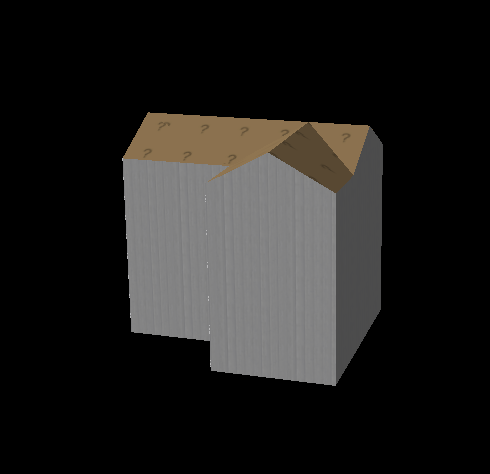
\includegraphics[scale=0.5]{figures/FixedByMe/3DFKBbuilding.png}
    \caption{3D representation of a FKB building, result of listing \ref{eq:3D_fkbbuilding}}
    \label{fig:3DFKBbuild}
\end{figure}




%The participants on the workshop agreed on building outlines should be used for the most general area of a complex building and building parts used to describe the special parts with different heights or other attributes, etc. As mentioned in section \ref{buildOSM}, the building outline should be tagged with building=* and building parts with building:part=*. Building outline is either a closed way or a multi-polygon and represents the area of land covered by the union of all building parts, the building footprint \cite{OSMwikipage2016}. Attributes like address, name, height, etc. must be tagged on the building outline. The building outline is important because it provides the compatibility for 2D rendering software. 2D renderers ignore building:part=* tags and only displaying the building outline. A relation tagged with type=building should be used if there are more than  one building part. This groups the building outline and all building parts together, as mentioned in section \ref{buildOSM}. 

There are different tools developed to visualizing 3D buildings with data from OSM. A problem is that not all tools supports the different modelling A list of which of them who supports the simple 3D building schema is located at the OSM simple 3D buildings wiki page, most tools accept this schema. 7 tools supports building:part=yes %http://wiki.openstreetmap.org/wiki/3D_Development/Tagging#Usage_Community
2D renderers ignore building:part=* tags, only displaying the building outline. 

An example of 3D building generated from FKB data is shown in listing xx. This use the simple 3D building schema. 

\section{Evaluation}



%\chapter{OSM comminity}

\subsection{Communication}
To communicate with users located all over the world, speaking different languages, is challenging. In OpenStreetMap users work together to create a high-resolution, global representation of the world. All the work done lies in a database which makes the communication and collaboration more challenging. During the Haiti earthquake a big problem was overlapping data. Three independent users could add the same road, with different tags, creating chaos on the map. Especially this event 


Generally in Open Source projects the communication between producers 

\subsection{Motivation}

%Chapter: Microtaskin, see paper: Success & Scale in a Data-Producing Organization s 4118, Org&ikt mappen.
% Tasking manager

%Chapter: FKB
%  About SOSI
%	 Data quality, how is the data produced
%	 Metadata - SOSI
%  Metadata - OSM, how is Trondheim covered today?
% 3D buildings Mapbox, how is the logic similair with SOSI?  https://www.mapbox.com/blog/mapbox-studio-building-heights/
	% Taking this (building) data as a start for 3D mapping of New York, several users have been 		refining roof-shapes and building parts data. http://wiki.openstreetmap.org/wiki/New_York_City#Possible_Imports
% 3D modeling OSM
	%http://wiki.openstreetmap.org/wiki/Roof_3D_modeling
	%http://wiki.openstreetmap.org/wiki/3D_modeling
	%http://wiki.openstreetmap.org/wiki/Simple_3D_buildings
	%http://forum.openstreetmap.org/viewtopic.php?id=32131
% Licence, not FKB public yet 
% Motivation: Tasking manager has statistics with, among others, a top-list of the most active contributors.  

%Suggested method for importing FKB to OSM 
	% Går tilbake til metodene, hva kan vi lære i Norge hvor vi ikke har Mapbox. Norske FKB er bedre enn de man har importert i andre land
	% Se på scriptene 
	% Her ta mappingen over til OSM , lua filen
	% Hvordan dele opp i tasking områder, telle antall hus. 50-30-20 hus innenfor hver task?
	% Dette er en utfordring, men er utenfor scopet til oppgaven. Komme med noen tanker rundt hvordan det kan løses. 
	
%\chapter{Summary of papers}

\subsection{Quality analysis of open street map data \cite{Wang2013}}\label{sec:wang}
Crowd sourcing geographic data is an opensource geographic data which is contributed by lots of non-professionals and provided to the public. Compared with conventional data collection and update methods, the crowd sourced geographic data has characteristics or advantages of large data volume, high currency, abundance information and low cost and becomes a research hotspot of international geographic information science in the recent years.\\ 
The primary problem is to analyse the quality of crowd sourcing geographic data. 
There are three factors that influence the quality of OSM: First data collected and mapped by non-professionals, secondly the collected data may be from different data sourcing with different precision and thirdly the data collected by different GPS may have different precisions. \\
The paper assesses three quality elements: 1. Data completeness, 2. Attribute accuracy and 3. Position accuracy. 

Enter twice to get spacing between paragraphs.

\paragraph{Data completeness}
Includes length completeness and name completeness. Length completeness is the geometric quality and data coverage. Formula: $Q_{L}=\frac{L_{OSM}}{L_{R}}$ \\(L = percentage of the length).  
\paragraph{Name completeness}
Name completeness means the completeness of the name attribute. 

\subsection{User generated Street Maps \cite{Weber2008}}\label{sec:weber}
Until recently the mapping of the Earth was preserved highly skilled, well-equipped and organized individuals and groups. The big change happened in 2000 when Bill Clinton removed the selective availability of the GPS signal, this provided much improved accuracy for simple, low-cost GPS receivers. The wide availability of high-quality location information has enabled mass-market mapping based on affordable GPS receivers, home-computers and the Internet. 
\paragraph{OSM background}
OSM follows the peer production model that created Wikipedia. Its aim is to create a set of map data thats free to use, editable, and licensed under new copyright schemes. Was founded in 2004 at University College London. In May 2008 OSM had more than 33,000 registered users and about 3,500 currently active contributors. OSM decided to follow the route of allowing only registered users to edit the map, this way they can trace the information source. OSM GeoStack is the set of tools that lets users capture, procedure, communicate, aggregate, and consume the geographical information produced in the project.  
\paragraph{Editing Tools}
OSM developers implement tools to facilitate user contributions to the database. In 2008 they had a Flash-based editor called Potlatch. Today JOSM is more common, even though this is used by more experienced OSM contributors. At the end of 2006, Yahoo granted OSM the right to use its satellite imagery to trace roads and other features. 

\subsection{\href{http://icaci.org/files/documents/ICC_proceedings/ICC2009/html/nonref/22_6.pdf}{CROWDSOURCING IS RADICALLY CHANGING THE GEODATA LANDSCAPE: CASE STUDY OF OPENSTREETMAP \cite{Chilton}}}\label{crowdsourcing}
Examining the effect of the changing cartography has on data collection using OSM crowdsourcing as a case study. Are parallels to what is happening with data collection in other aspects, like WIKIPEDIA, Flickr and YouTube. \\

	- Today: A need for instant information, particularly in crisis situations\\
	- User Generated Content providers / crowdsourced data collectors are allowed to collect geodata\\
		- Reason: More available satellite imagery, cheaper GPS units, etc \\
		- OSM the leading global example \\
		- OSM was the first online mapping service to accurately map and display the new London Heathrow Terminal 5, on the official opening day. \\
	- OSM project \href{http://wiki.openstreetmap.org/wiki/No:Main_Page} - the achieved coverage, its accuracy, availability and global impact are all changing the way individuals and org are thinking about the collection, purchase and use of geodata. \\
	- Makes OSM stand out from other data sources: \\
		- Completely free of charge \\
		- Is released under a license which allows you to do pretty much what you like \\
			As long as you mention the original creator and the license 
			\href{http://wiki.openstreetmap.org/wiki/OpenStreetMap_License} \\
	- The availability, accuracy and price of OSM data has lead some local authorities in the UK to question the need to have total reliance on being locked into a contract for their geodata with the National Mapping Agency. \\
	- OSM gives the possibility of having really current data available, other services may have a large lead for getting the data from survey to map output. \\
OSM have specialist maps for cycling, routing, applications, skiing, topography and for maritime use. 

\subsection{\href{http://www.giscience2010.org/pdfs/paper_213.pdf}{The impact of crowdsourcing on spatial data quality indicators}}
Introduce the concept "Crowd Quality" (CQ) to describe and quantify the quality of crowdsourced geospatial information. Together with the growth in volume, the usage of crowdsourced geospatial info. grew extensively as well.

	- Quality: Has a meaning if we have a common understanding of its definition \\
		 - ISO19113(2002): Quality is the "totality of characteristics of a product that bear on its ability to satisfy stated and implied needs".  \\
	 - Van Oort: Identified eleven elements of spatial data quality. The elements are used to describe the quality of geo-data collected and produced. \\
	  -  Uniform method to produce and process the data --> Homogenous and consistent quality \\
	- Crowd Quality (CQ): \\
		- 2 dim.: \\
			1. User-related quality aspects: Quality of information from an individual contributors perspective. This is the typical char. of crowdsourced data.\\
			2. Feature-related quality aspects: Perspective of the spatial feature. \\
			
	1. 3 components: Local Knowledge, Experience and Recognition. \\
		a. Familiarity to an area can be correlated to the quality of the users contribution \\
		b. Quality of a users contribution is correlated with his overall experience in contributing to the project \\
		c. Online social networks that allow for user contributions, often feedback are established (ratings, recognition for specific contributions). This type of User recognition is largely unknown in crowdsourced geospatial data --> Puts a strain in our ability to assess CQ. \\
	2. In crowdsources datasets quality elements can be different for similar features, one user can add his personal attributes when adding a restaurant in OSM, while another restaurant only have one attribute. In traditional datasets the quality elements will be uniform, have the same attributes. \\ 
		a. Quality elements that are particular interesting, since they are not consistent for crowdsourced data: \\
			1. Lineage, positional accuracy and sematic accuracy.  \\
			When data is imported from other sources, these imported features have a very clear lineage with regard to positional accuracy and precision. When imported from GPS data, the positional accuracy is harder to establish. \\
Sematic accuracy  - related to the completeness and internal consistency of the attribute metadata. A schema for attribute metadata is not common in crowdsources geospatial data projects --> Create a threat to internal consistency. 

\chapter{Movies}
\subsection{\href{http://stateofthemap.us/2015/less-bots-more-humans-using-maproulette-to-import-data/}{State of the Map, microtasking}}\label{sec:movie}
A bot is a tool that carries out repetitive and mundane (dagligdagse) automated edits on a regular basis to help maintain OSM. Most bots deal with tagging, ex xybot. BugBuster deals with removing nodes. Czechreg deals with changing geometries. 

Issues with importing: The person need to have experience with the tool and the data, but also need to have the time to manually verify each task. Therefore we have microtasking - A process of splitting a task into multiple subtasks and distributing these subtasks to humans over the internet. He things this is the way of the future. Breaking up tasks tools - OSMLY, MapRoulette, BattleGrid. They can solve our issue, but we need different tools. One to determine conflicting objects,  saving the tasks in a backend and then make a usable and easy frontend to work on the tools. \href{http://wiki.openstreetmap.org/wiki/OSM_Tasking_Manager}{OSM Tasking manager, divide up a mapping job}.

Microtasked conflation may lead to standard procedures that can help other groups import data.  Can help provide a validation step to force someone to look at each and every contribution. 

%Kommersielle bidragsytere, de har selv nytte av det

%Konklusjon - hvorfor gjør du dette
	% 

\bibliographystyle{apalike}
\bibliography{prosjektoppg.bib}


\chapter{Source - OSM mailing lists}
The mailing lists and threads used as information source in this paper.\\ 
\begin{enumerate}
 \item NUUG kart, mailing threads: \label{mail:nuugkart} 
 	\begin{itemize}
 		 \item sosi2osm \cite{Gnonthgol2013}
 		 \item Bruk av datasett fra Kartverket i OpenStreetMap \cite{Kihle2014}
 		 \item Moesvatn \cite{Didriksen2014}
 	\end{itemize}
 \item OSM-talk, mailing threads: \label{mail:osmtalk}
 	 \begin{itemize}
 		\item TIGER upload status since 0.5 api \cite{Munro2007}
 		\item TIGER, which states next? \cite{Mielczarek2007}
 		\item TIGER update (need more suggestions) \cite{Hansen2007b}
 		\item TIGER upload queue (maps of entire US) \cite{Hansen2007}
 	\end{itemize}
 \item Imports, mailing threads: \label{mail:imports}
 	 \begin{itemize}
 		 \item N50 imports from Kartverket \cite{Mehus2014}
 	\end{itemize}
 \end{enumerate} 
 
 \chapter{Appendix}

\lstset{
    language=XML,
    morekeywords={encoding,node, tag},
    label=eq:3D_fkbbuilding,
    caption=Example of a 3D representation of a house from FKB data in OSM XML. 
}
\begin{lstlisting}
<node id="-161645" lat="63.4485538" lon="10.1827768" version="1" visible="true"/>
	<node id="-387759" lat="63.4485656" lon="10.1827249" version="1" visible="true"/>
	<node id="-387760" lat="63.4484758" lon="10.1826237" version="1" visible="true"/>
	<node id="-387761" lat="63.4484641" lon="10.1826756" version="1" visible="true"/>
	<node id="-387762" lat="63.4484517" lon="10.1827306" version="1" visible="true"/>
	<node id="-387763" lat="63.4484944" lon="10.1827787" version="1" visible="true"/>
	<node id="-387764" lat="63.4484820" lon="10.1828337" version="1" visible="true"/>
	<node id="-387765" lat="63.4485052" lon="10.1828598" version="1" visible="true"/>
	<node id="-387766" lat="63.4485289" lon="10.1828866" version="1" visible="true"/>
	<node id="-387767" lat="63.4485411" lon="10.1828332" version="1" visible="true"/>
	<way id="-166806" version="1" visible="true">
		<tag k="OMRÅDEID" v="1601"/>
		<tag k="KVALITET" v="24; 19; 0; 24; 23"/>
		<tag k="TRE_D_NIVÅ" v="2"/>
		<tag k="KURVE" v="166806"/>
		<tag k="OBJTYPE" v="Takkant"/>
		<tag k="building" v="yes" />
		<tag k="height" v="12.80" />
		<tag k="roof:height"  v="4"/>
		<tag k="building:colour" v="white"/>
  		<tag k="building:material" v="wood"/>
		<nd ref="-161645" />
		<nd ref="-387759" />
		<nd ref="-387760" />
		<nd ref="-387761" />
		<nd ref="-387762" />
		<nd ref="-387763" />
		<nd ref="-387764" />
		<nd ref="-387765" />
		<nd ref="-387766" />
		<nd ref="-387767" />
		<nd ref="-161645" />
	</way>
	<node id="-161645" lat="63.4485538" lon="10.1827768" version="1" visible="true"/>
	<node id="-59094" lat="63.4485300" lon="10.1827499" version="1" visible="true"/>
	<way id="-59454" version="1" visible="true">
		<tag k="OMRÅDEID" v="1601"/>
		<tag k="KVALITET" v="24; 19; 0; 24; 23"/>
		<tag k="TRE_D_NIVÅ" v="2"/>
		<tag k="KURVE" v="59454"/>
		<!-- <tag k="building:part" v="yes"/> -->
		<!-- <tag k="roof:angle" v="-30" />  -->
		<!-- <tag k="roof:shape" v="gabled"/> -->
		<tag k="OBJTYPE" v="Mønelinje"/>
		<tag k="height" v="18.28" />
		<tag k="roof:height"  v="1.57"/>
		<tag k="roof:ridge" v="yes" />
		<tag k="roof:colour" v="#d162ac"/>
		<tag k="roof:material" v="brick"/>
		<nd ref="-161645" />
		<nd ref="-59094" />
	</way>
	<node id="-161646" lat="63.4484641" lon="10.1826756" version="1" visible="true"/>
	<way id="-59455" version="1" visible="true">
		<tag k="OMRÅDEID" v="1601"/>
		<tag k="KURVE" v="59455"/>
		<tag k="OBJTYPE" v="Mønelinje"/>
		<tag k="height" v="18.28" />
		<tag k="roof:height" v="1.57"/>
		<tag k="roof:ridge" v="yes" />
		<tag k="roof:colour" v="#d162ac"/>
		<tag k="roof:material" v="metal"/>
		<nd ref="-59094" />
		<nd ref="-161646" />
	</way>
	<node id="-161633" lat="63.4485052" lon="10.1828598" version="1" visible="true"/>
	<way id="-59447" version="1" visible="true">
		<tag k="OMRÅDEID" v="1601"/>
		<tag k="ORIGINALDATAVERT" v="Trondheim kommune"/>
		<tag k="KURVE" v="59447"/>
		<tag k="OBJTYPE" v="Mønelinje"/>
		<tag k="height" v="18.28" />
		<tag k="roof:height" v="1.57"/>
		<tag k="roof:ridge" v="yes" />
		<tag k="roof:colour" v="#d162ac"/>
		<tag k="roof:material" v="brick"/>
		<nd ref="-59094" />
		<nd ref="-161633" />
	</way>
	<node id="-59093" lat="63.4485411" lon="10.1828332" version="1" visible="true"/>
	<node id="-59094" lat="63.4485300" lon="10.1827499" version="1" visible="true"/>
	<node id="-59095" lat="63.4484944" lon="10.1827787" version="1" visible="true"/>
	<way id="-21118" version="1" visible="true">
		<tag k="OMRÅDEID" v="1601"/>
		<tag k="KURVE" v="21118"/>
		<tag k="OBJTYPE" v="Bygningslinje"/>
		<tag k="roof:edge" v="yes" />
		<tag k="roof:colour" v="#78d162"/>
		<tag k="roof:material" v="brick"/>
		<nd ref="-59093" />
		<nd ref="-59094" />
		<nd ref="-59095" />
	</way> 
\end{lstlisting}

	

\end{document}  
